\chapter{Estudi d'Experiència d'Usuari (UX)}

\section{Anàlisi}
L'objectiu d'aquest apartat és definir com seran els usuaris potencials de l'aplicació. Per a fer-ho s'analitzarà com interaccionen amb les aplicacions de gestió de despeses per extreure les necessitats i els requeriments del producte.

\subsection{Investigació contextual}
En aquesta secció s'ha estudiat com els usuaris gestionen les despeses. Per a fer-ho, s'han entrevistat 9 usuaris sobre com gestionen actualment les seves despeses, demanant que mostressin com ho feien. A més a més, a 4 d'aquests 9 usuaris se'ls ha demanat que utilitzessin varies aplicacions ja existents al mercat (\gls{Google_play}). Un cop les feien servir en directe se'ls preguntava quines coses els havien agradat i quines no. 
%TODO link apps

La totalitat de l'entrevista ha estat transcrita al moment i conduïda per la plantilla de la figura \ref{fig:plantilla_analisi}. És important remarcar que tot i ser una entrevista es buscava, sempre que era possible, que els usuaris mostressin com treballen, enlloc de que expliquessin amb paraules com ho fan. També, quan els usuaris utilitzaven les aplicacions s'ha gravat un vídeo amb el què veien a la pantalla mentre feien servir les aplicacions així com el que poguessin estar dient en aquell moment. L'objectiu de fer aquestes gravacions és facilitar, si s'escau, el posterior anàlisi per aclarir parts de l'enquesta que no fossin prou clars. Al comptar amb so, també ha servit per localitzar i identificar les funcions o apartats que frustraven o motivaven als usuaris. Per últim, quan ha estat possible s'han recol·lectat imatges o documents que ensenyessin com els usuaris gestionen les seves despeses i/o ingressos. 

\begin{figure}[htp]
\centering
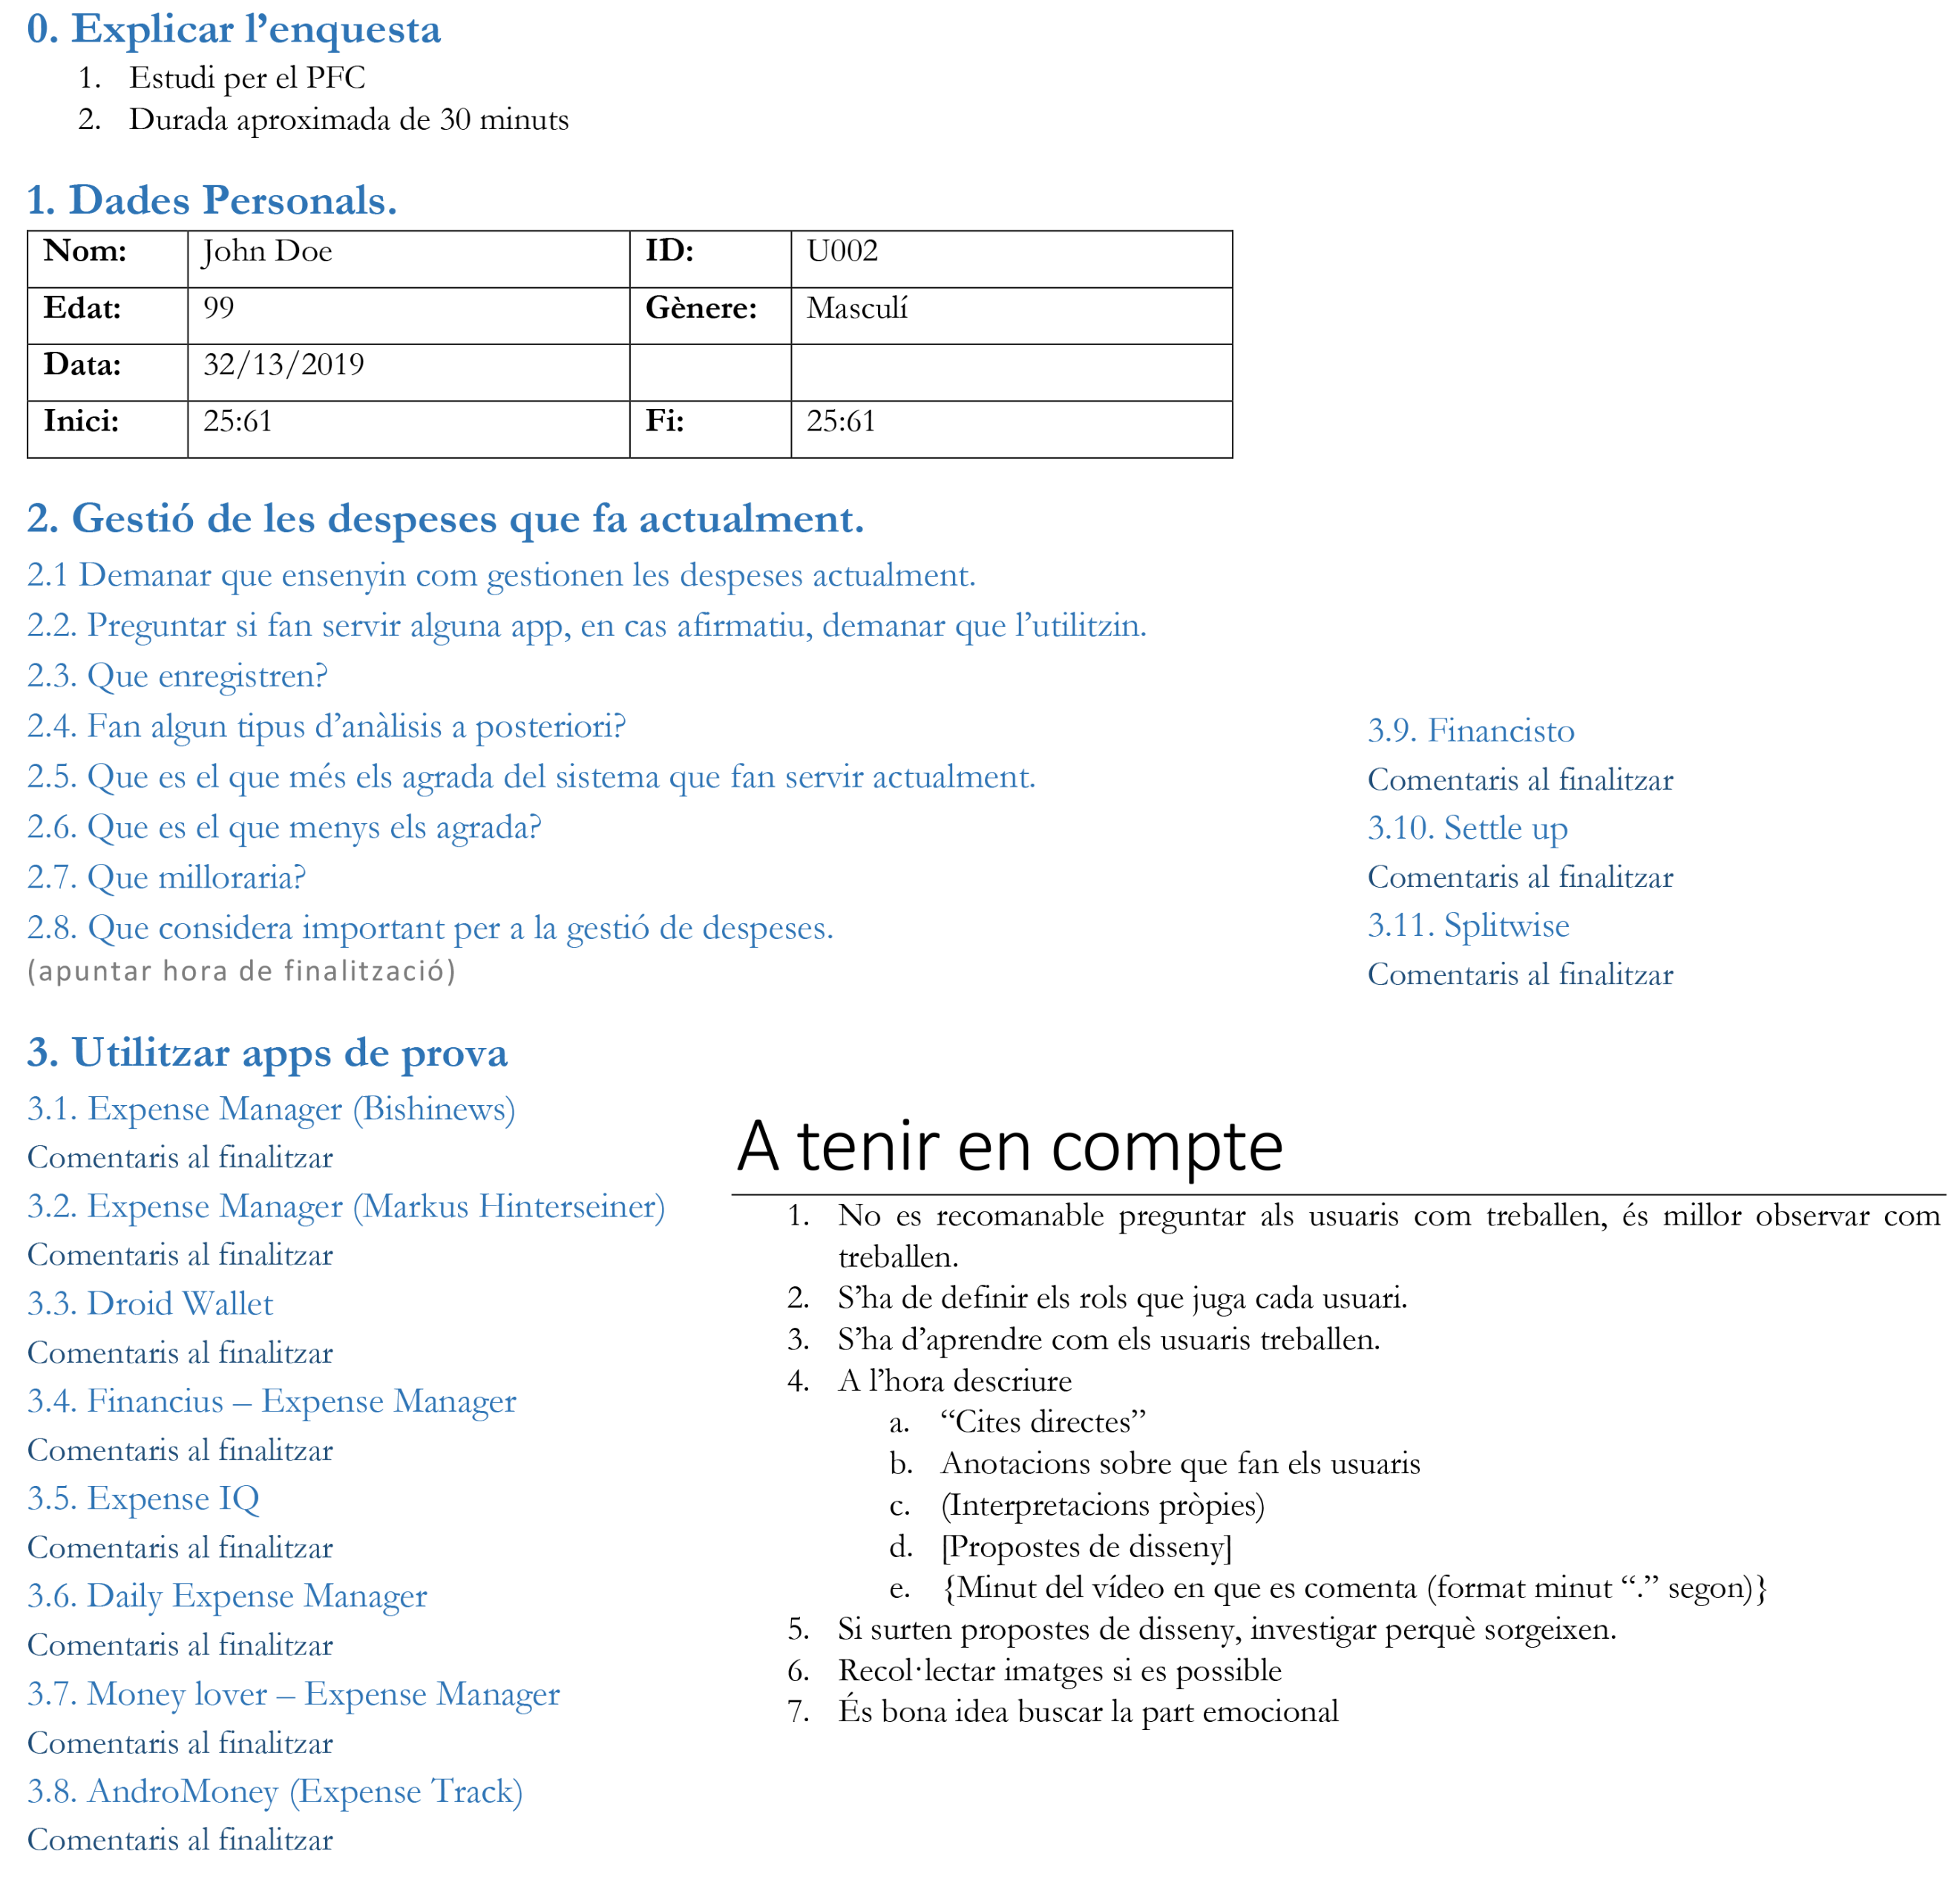
\includegraphics[scale=0.65]{plantilla_analisi.png}
\caption{Plantilla emprada a la investigació contextual}\label{fig:plantilla_analisi}
\end{figure}

\subsection{Anàlisi contextual}
En aquesta secció s'ha creat el model de flux (figura \ref{fig:flow_model}). També s'ha sintetitzat la informació extreta a la investigació contextual en \glspl{workActivityNotes}. Després amb les \glspl{workActivityNotes} s'ha creat el \ac{WAAD}, de manera que aquest mostra de manera clara i concisa la informació que s'ha extret dels usuaris. Cada \gls{workActivityNotes} dins del \ac{WAAD} està etiquetada amb el numero de nota i un identificador (format per lletres i números) que la posiciona dins el \ac{WAAD}.

%TODO link del WAAD

\begin{figure}[htp]
\centering
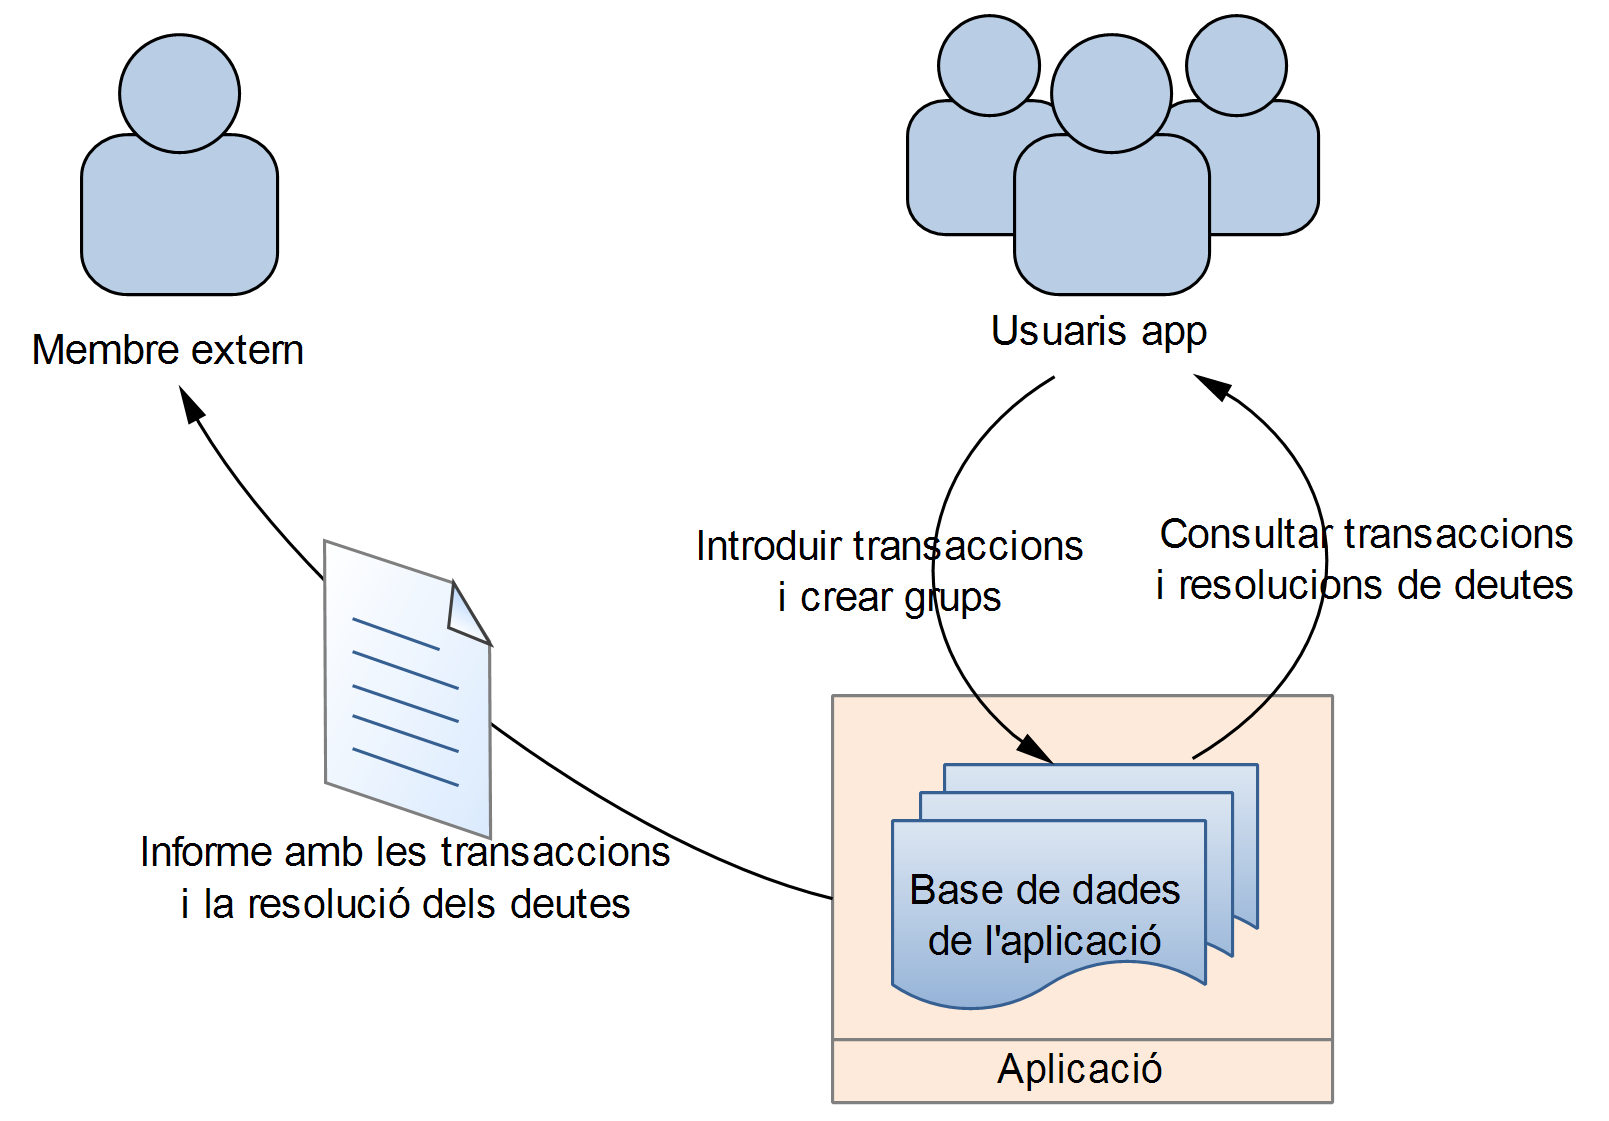
\includegraphics[scale=0.5]{flow_model.png}
\caption{Model de flux}\label{fig:flow_model}
\end{figure}

\subsection{Extracció dels requeriments d'interacció}
Aquí s'han extret els requeriments d'interacció a partir del \ac{WAAD}. A més a més, tal com recomana Rex Hartson (2012, p.168) \cite{UX_Book} també s'han inclòs de color verd els requeriments del sistema. S'han marcat amb un triangle (\blacktriangle) els requeriments més importants per tal de ressaltar-ne la seva importància. També, com que sovint l'usuari no menciona les coses que considera obvies, s'han extrapolat aquells requeriments que no estaven mencionats directament però que els usuaris esperen. 
Per últim, per a poder localitzar la font de cada requeriment, s'ha etiquetat entre claudàtors l'identificador del \ac{WAAD} de la \gls{workActivityNotes} de la qual prové.

\subsection{Construcció de models informatius per al disseny}
En aquesta secció s'han creat els diversos models descrits a l'apartat \ref{subsubsec:Construccio_models}.
Tot i això, com que el producte que s'està dissenyant és una aplicació per a \glspl{smartphone} no s'ha creat ni el Model d'artefacte ni el model físic, ja que cap dels dos aporta informació útil en aquest cas. 

\section{Disseny}
En aquesta etapa s'ha anat dissenyant i conformant la aplicació. Per a fer-ho primer s'han creat els personatges Rex Cooper i Maria Gestalt, com a usuari de l'aplicació i com a membre extern d'un grup respectivament,

\subsubsection{Rex Cooper}

En Rex és un jove de vint i llargs anys que està acabant els seus estudis de periodisme. Apart d’estudiar, en Rex treballa els matins de secretari. Com que durant la setmana gairebé no té temps per a dedicar al lleure, aprofita els caps de setmana per a quedar amb els seus amics i fer excursions a la muntanya. 
Actualment té uns ingressos baixos, per això intenta controlar les seves despeses i veure si arriba bé a final de mes. Si bé és cert que apunta la majoria de transaccions que fa, d'aquestes només apunta el més bàsic, com la quantitat i la categoria, ja que en general, ni té temps ni vol dedicar-hi gaire a enregistrar i estudiar les seves transaccions. Tot i això quan durant una època veu que va molt just econòmicament si que es dedica a apuntar amb més detall les seves despeses.

\begin{figure}
	\centering
	\begin{subfigure}[b]{0.5\textwidth}
		\centering
		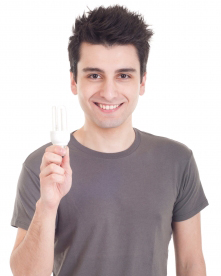
\includegraphics[scale=0.4]{Rex_cooper.jpg}
		\caption{Rex Cooper. Autor: Artur84}
		\label{fig:rex_cooper}
	\end{subfigure}
	\quad
	\begin{subfigure}[b]{0.5\textwidth}
		\centering
		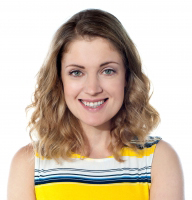
\includegraphics[scale=0.5]{Maria_gestalt.jpg}
		\caption{Maria Gestalt. Autor: stockimages}
		\label{fig:maria_gestalt}
	\end{subfigure}

\caption{Personatges creats. Imatges de: \url{http://www.freedigitalphotos.net/}}\label{fig:personas}
\end{figure}


\subsubsection{Maria Gestalt}

La Maria és una jove de gairebé 30 anys que treballa de monitora en un gimnàs. A més, a la Maria li agrada molt viatjar i sempre que pot aprofita per fer-ho amb els seus amics.
La Maria no està gaire interessada en els “números” i la comptabilitat, a més arriba a final de més (econòmicament) sense masses problemes. És per això que no vol enregistrar les seves despeses/ingressos. Però quan viatja això canvia, està acostumada a que els seus amics apuntin les despeses compartides que fan i que al acabar el viatge li diguin quants diners li deu (o deuen) i a quin dels seus amics. Quan li diuen només inverteix una estona a comprovar que no li hagin sumat alguna despesa de les quals no a participat. 

\paragraph{•}
Un cop creats els personatges s'ha començat a dissenyar. En les primeres iteracions el disseny s'ha efectuat a ma alçada, fent servir només unes plantilles rectangulars que simulaven la pantalla. A mesura que es refinava el disseny s'ha fet el canvi de fet a mà a fet amb ordinador. S'ha fet servir el programa \gls{Balsamiq_Mockups} (https://balsamiq.com/) ja que permet fer dissenys que simulen una aparença de baixa fidelitat, d'aquesta manera es garanteix que els usuaris no tinguin por de criticar el disseny (veure secció \ref{subsec:implementation}). Finalment, a les últimes iteracions s'ha passat a dissenys detallats al píxel fent servir el programa \gls{Android_Studio}. Es pot veure l'evolució dels dissenys a les taules \ref{table:images_app1}, \ref{table:images_app2} i \ref{table:images_app3}.

\begin{table}
\caption{Imatges de l'aplicació a les diverses etapes del disseny 1}
\label{table:images_app1}
\begin{tabular}{| c | c | c |}
\hline
Esbossos & Disseny Conceptual - intermedi & Disseny detallat - refinat \\
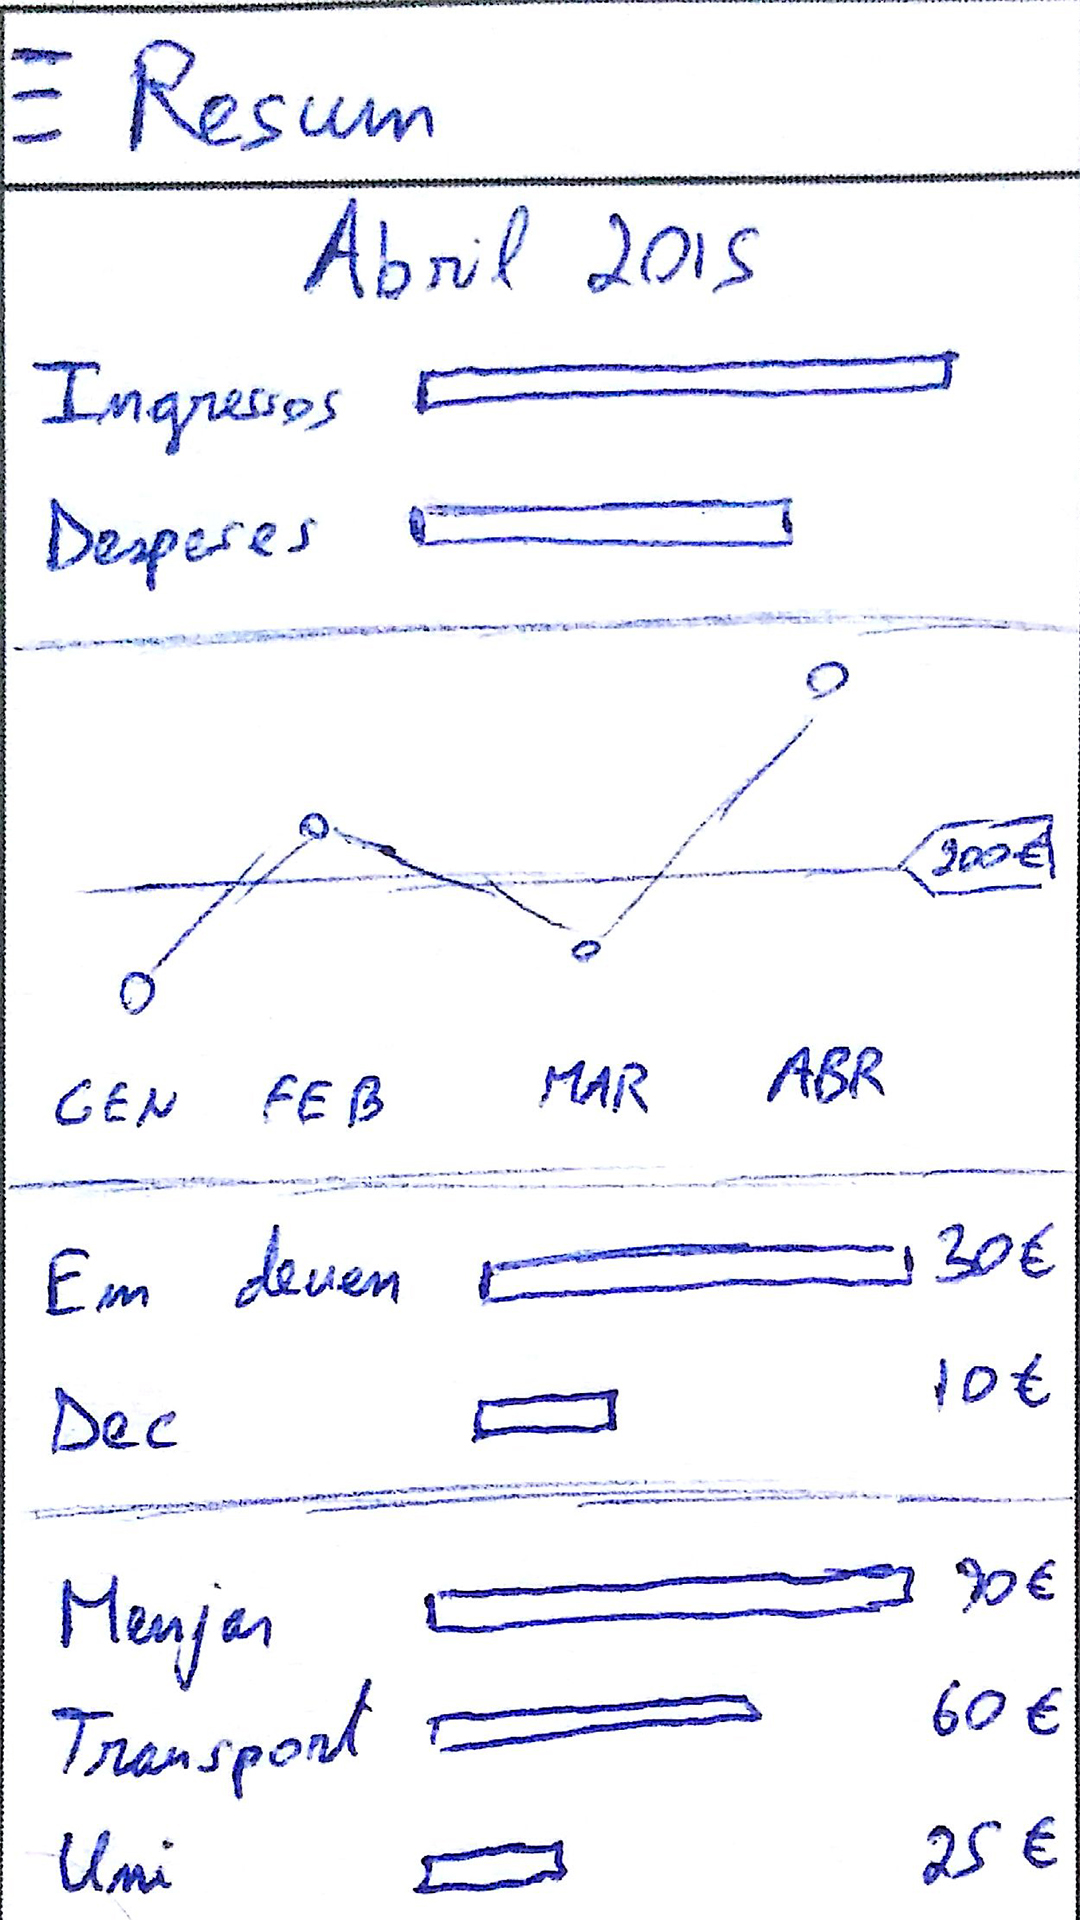
\includegraphics[width=50mm]{1_Dashboard.jpg} &
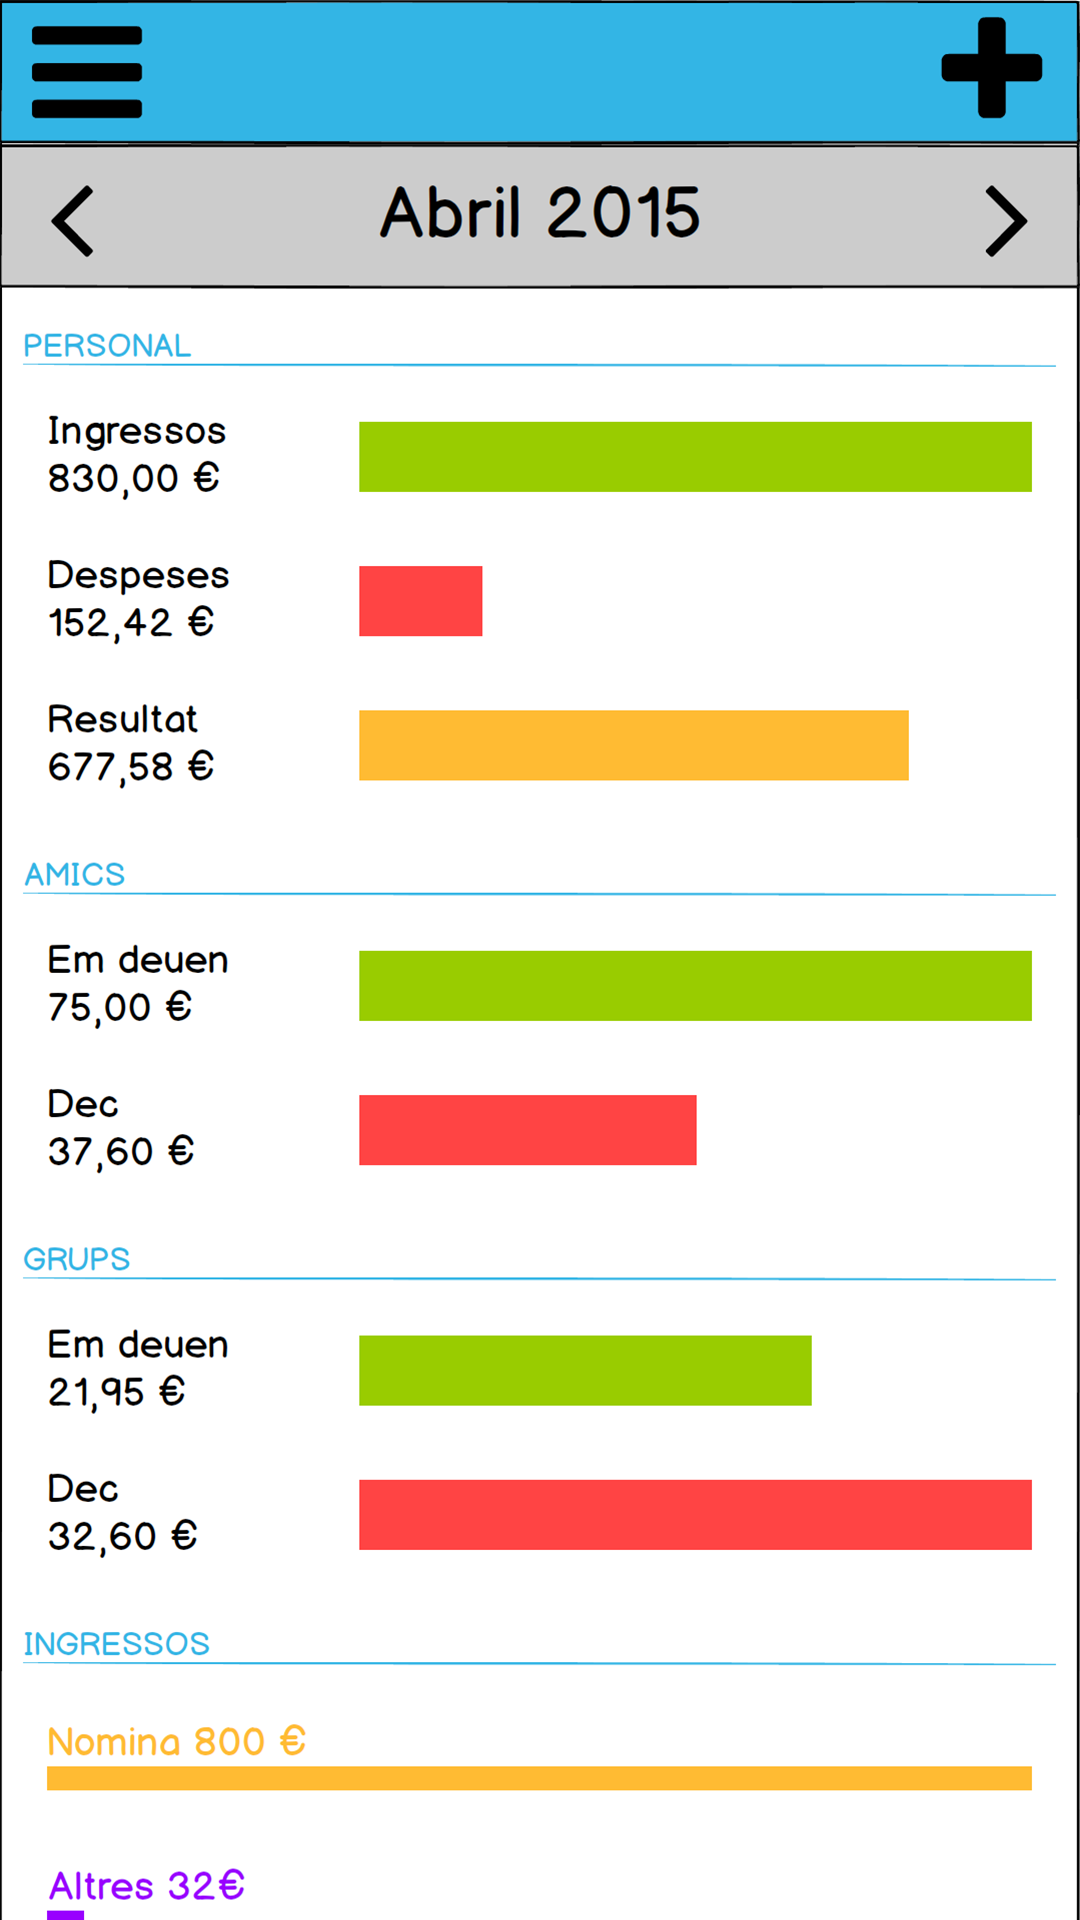
\includegraphics[width=50mm]{2_Dashboard.png} &
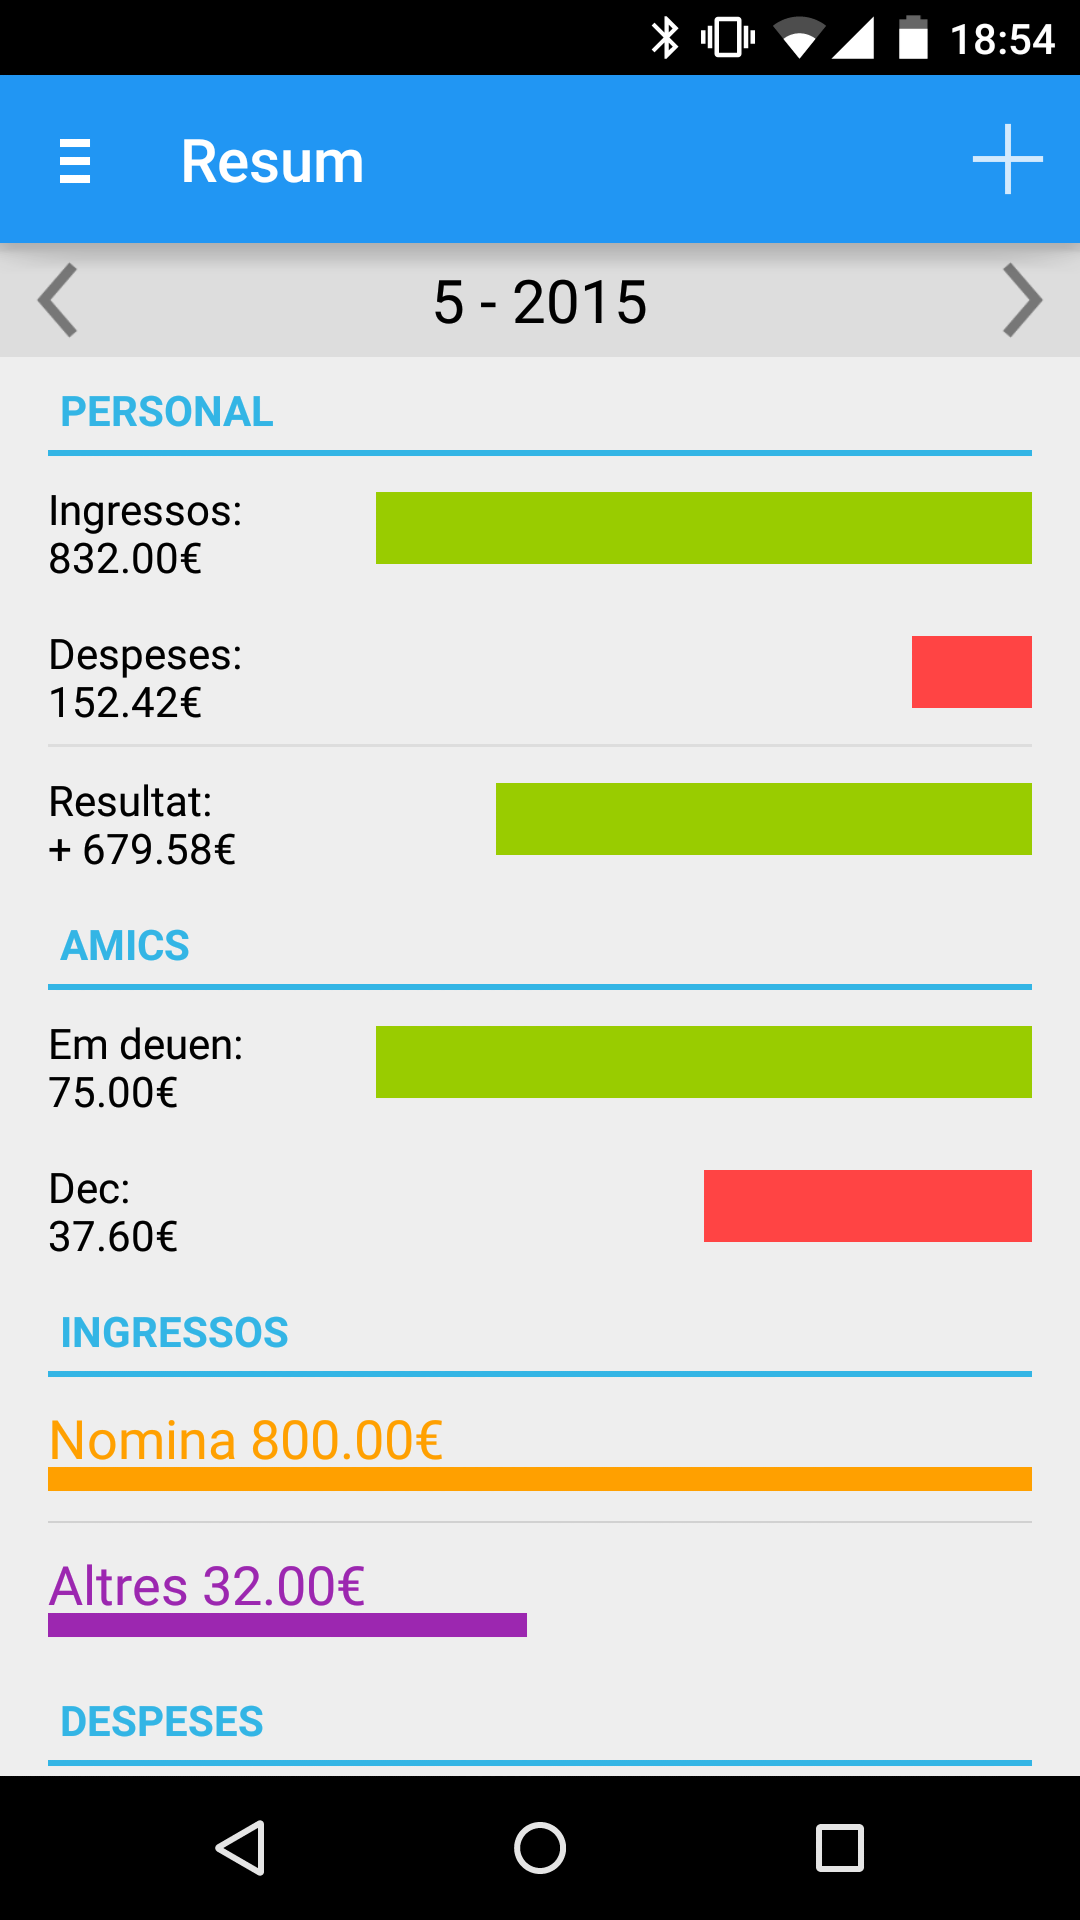
\includegraphics[width=50mm]{3_Dashboard.png} \\
\hline
Esbossos & Disseny Conceptual - intermedi & Disseny detallat - refinat \\
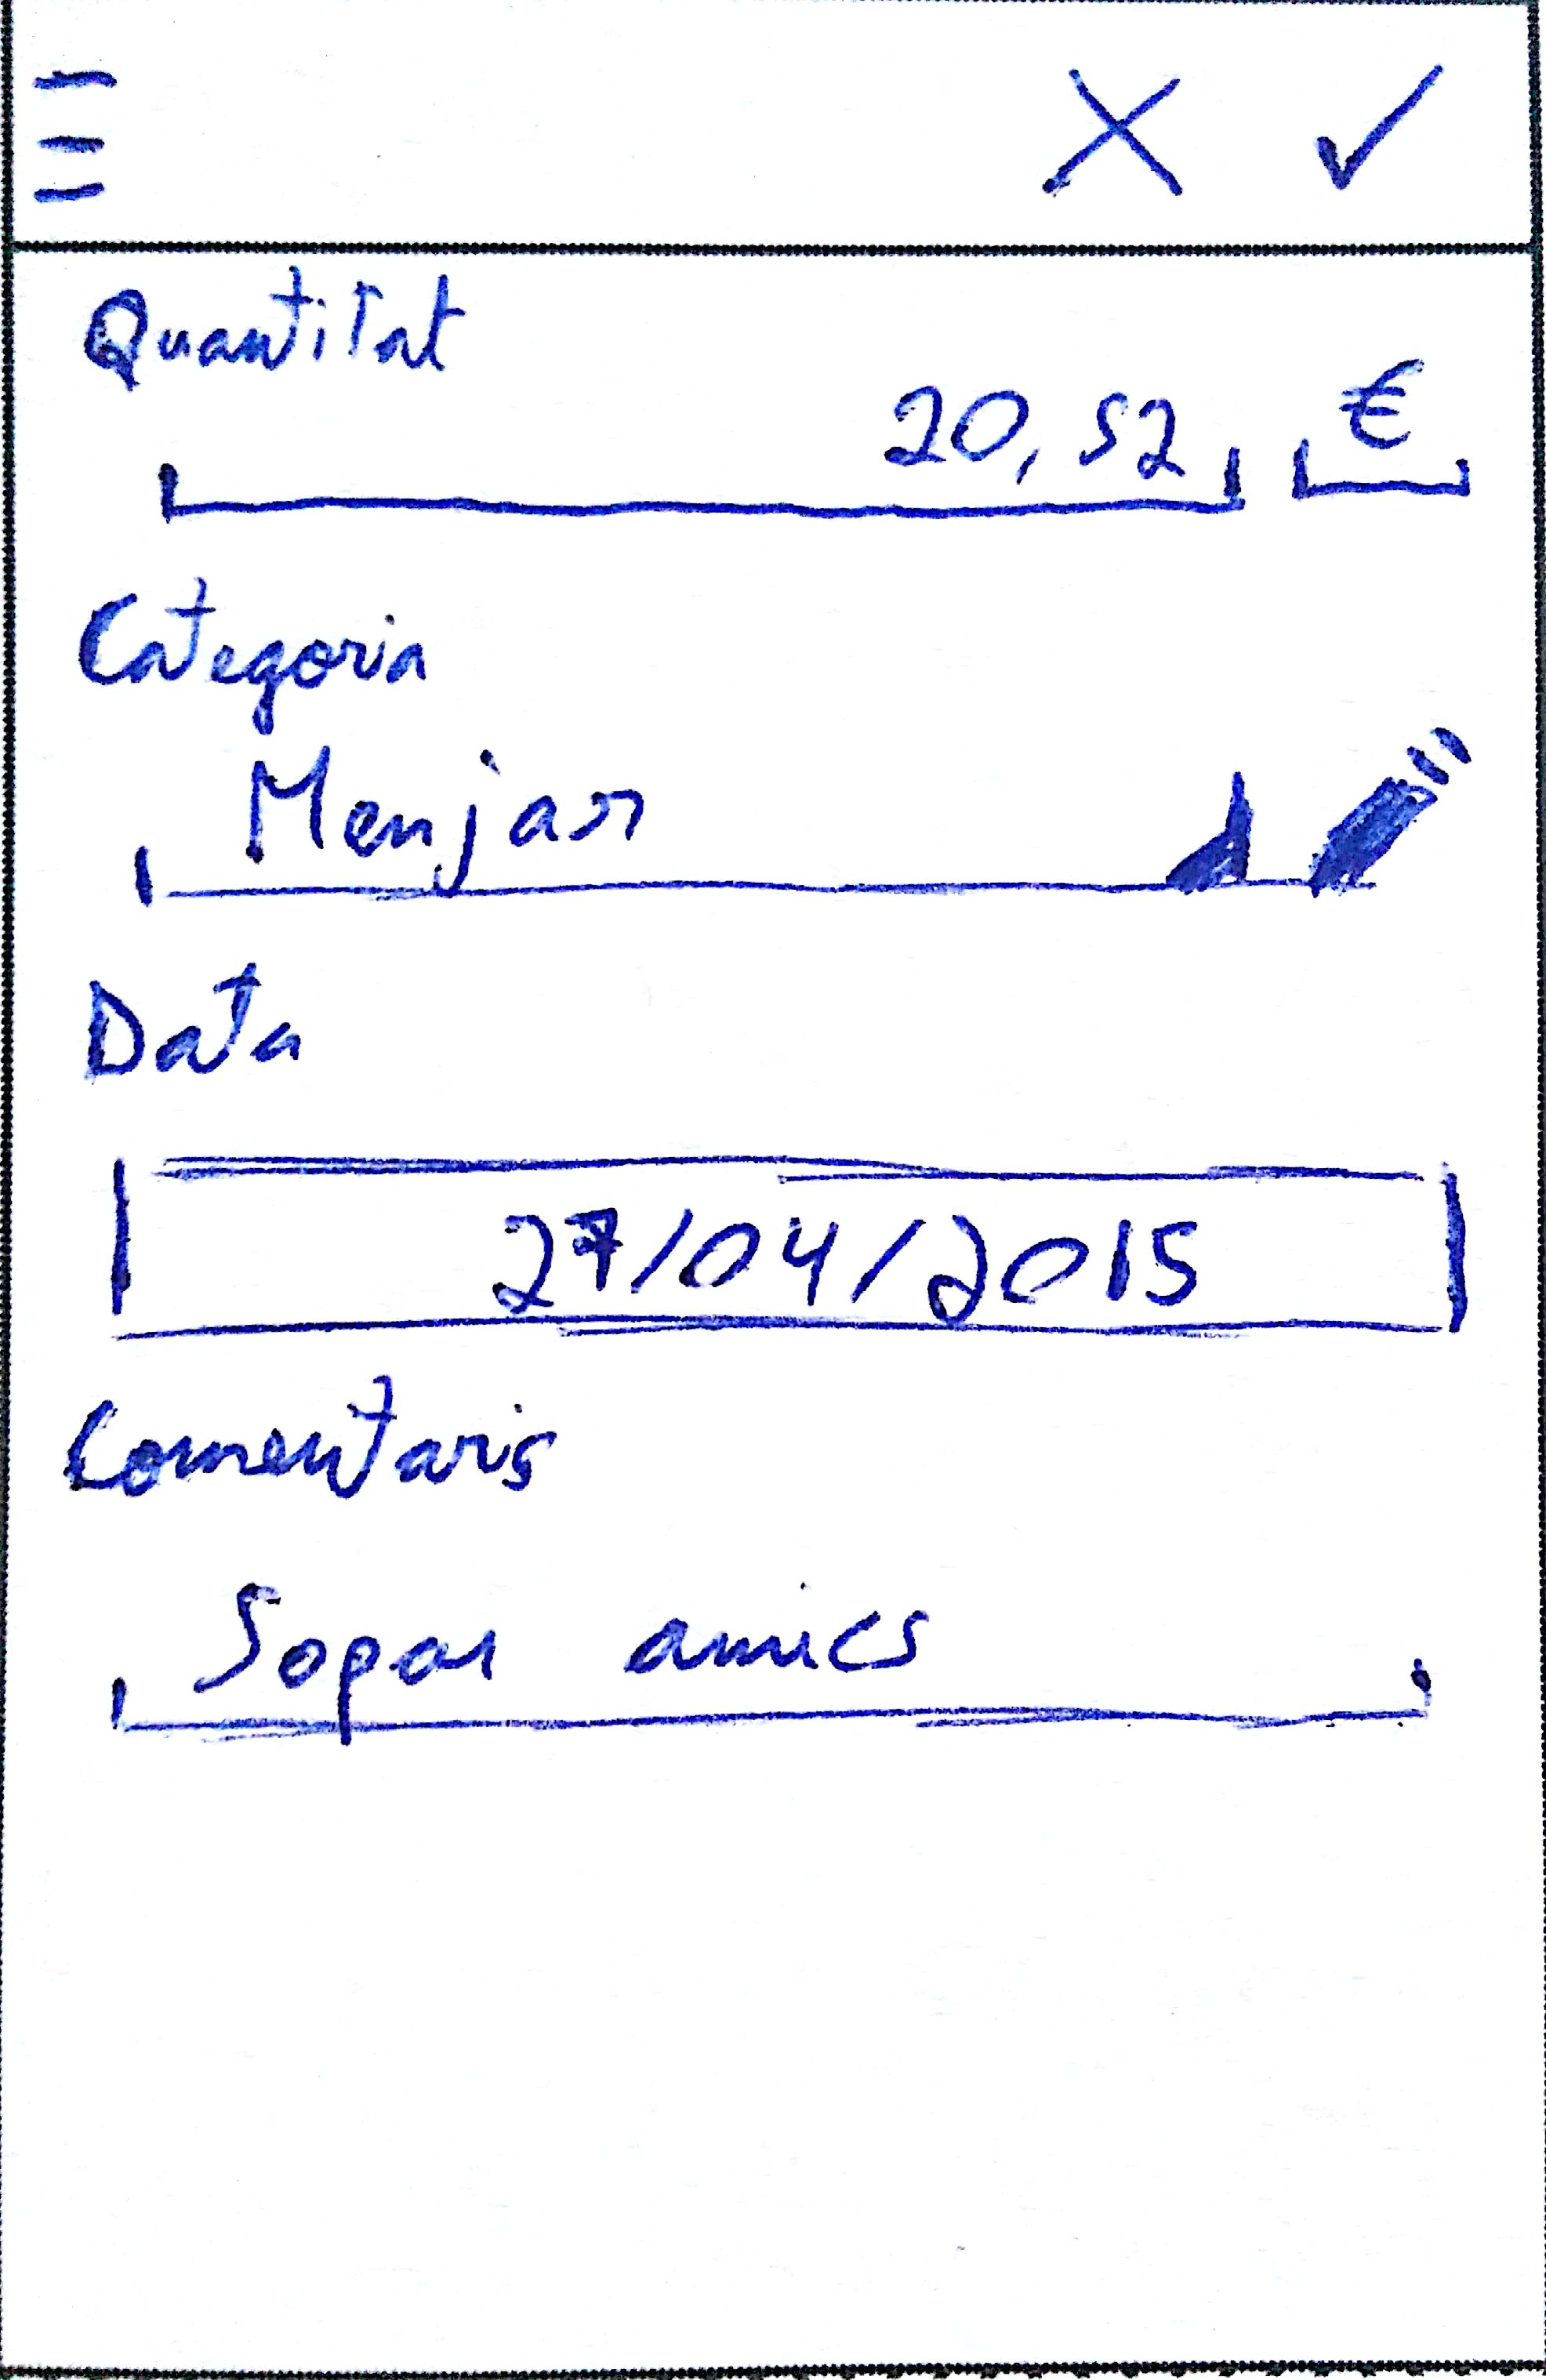
\includegraphics[width=50mm]{1_Add_expense.jpg} &
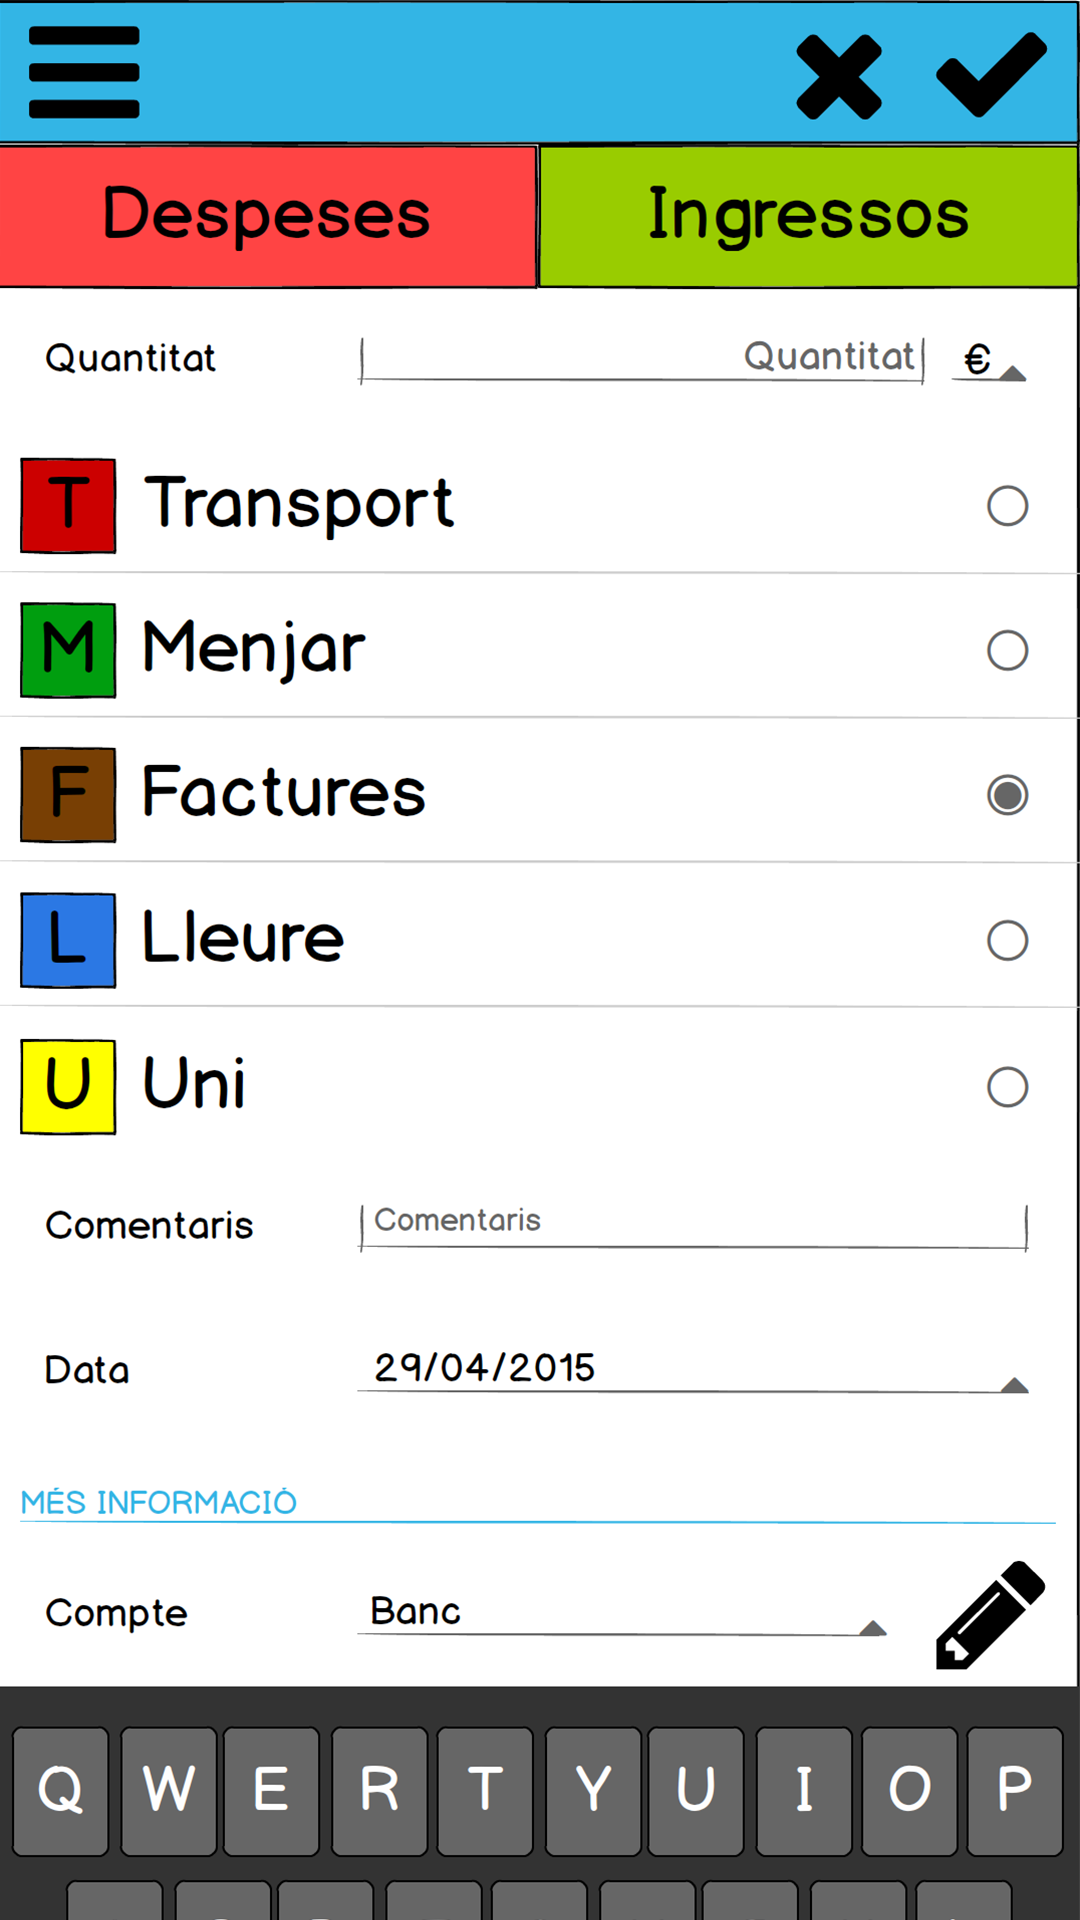
\includegraphics[width=50mm]{2_Add_expense.png} &
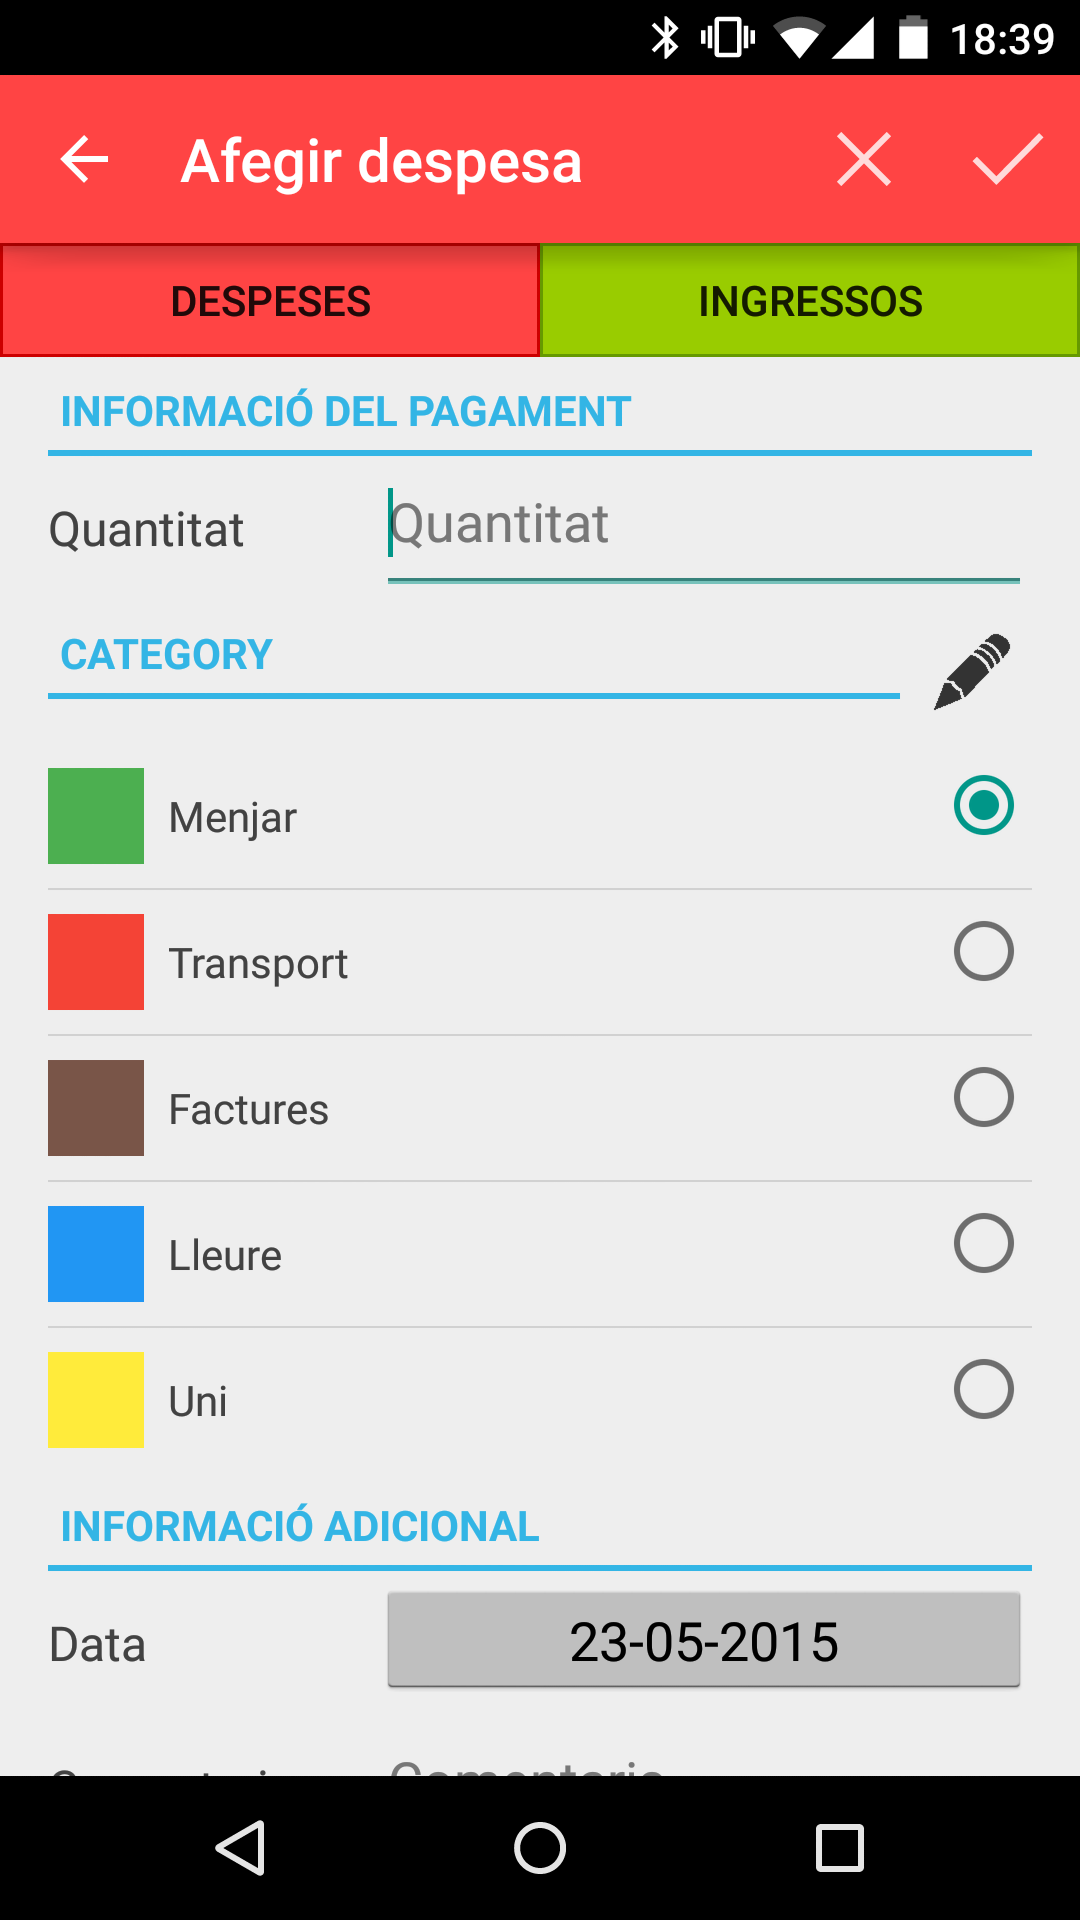
\includegraphics[width=50mm]{3_Add_expense.png} \\
\hline
\end{tabular}
\end{table}

\begin{table}
\caption{Imatges de l'aplicació a les diverses etapes del disseny 2}
\label{table:images_app2}
\begin{tabular}{| c | c | c |}
\hline
Esbossos & Disseny Conceptual - intermedi & Disseny detallat - refinat \\
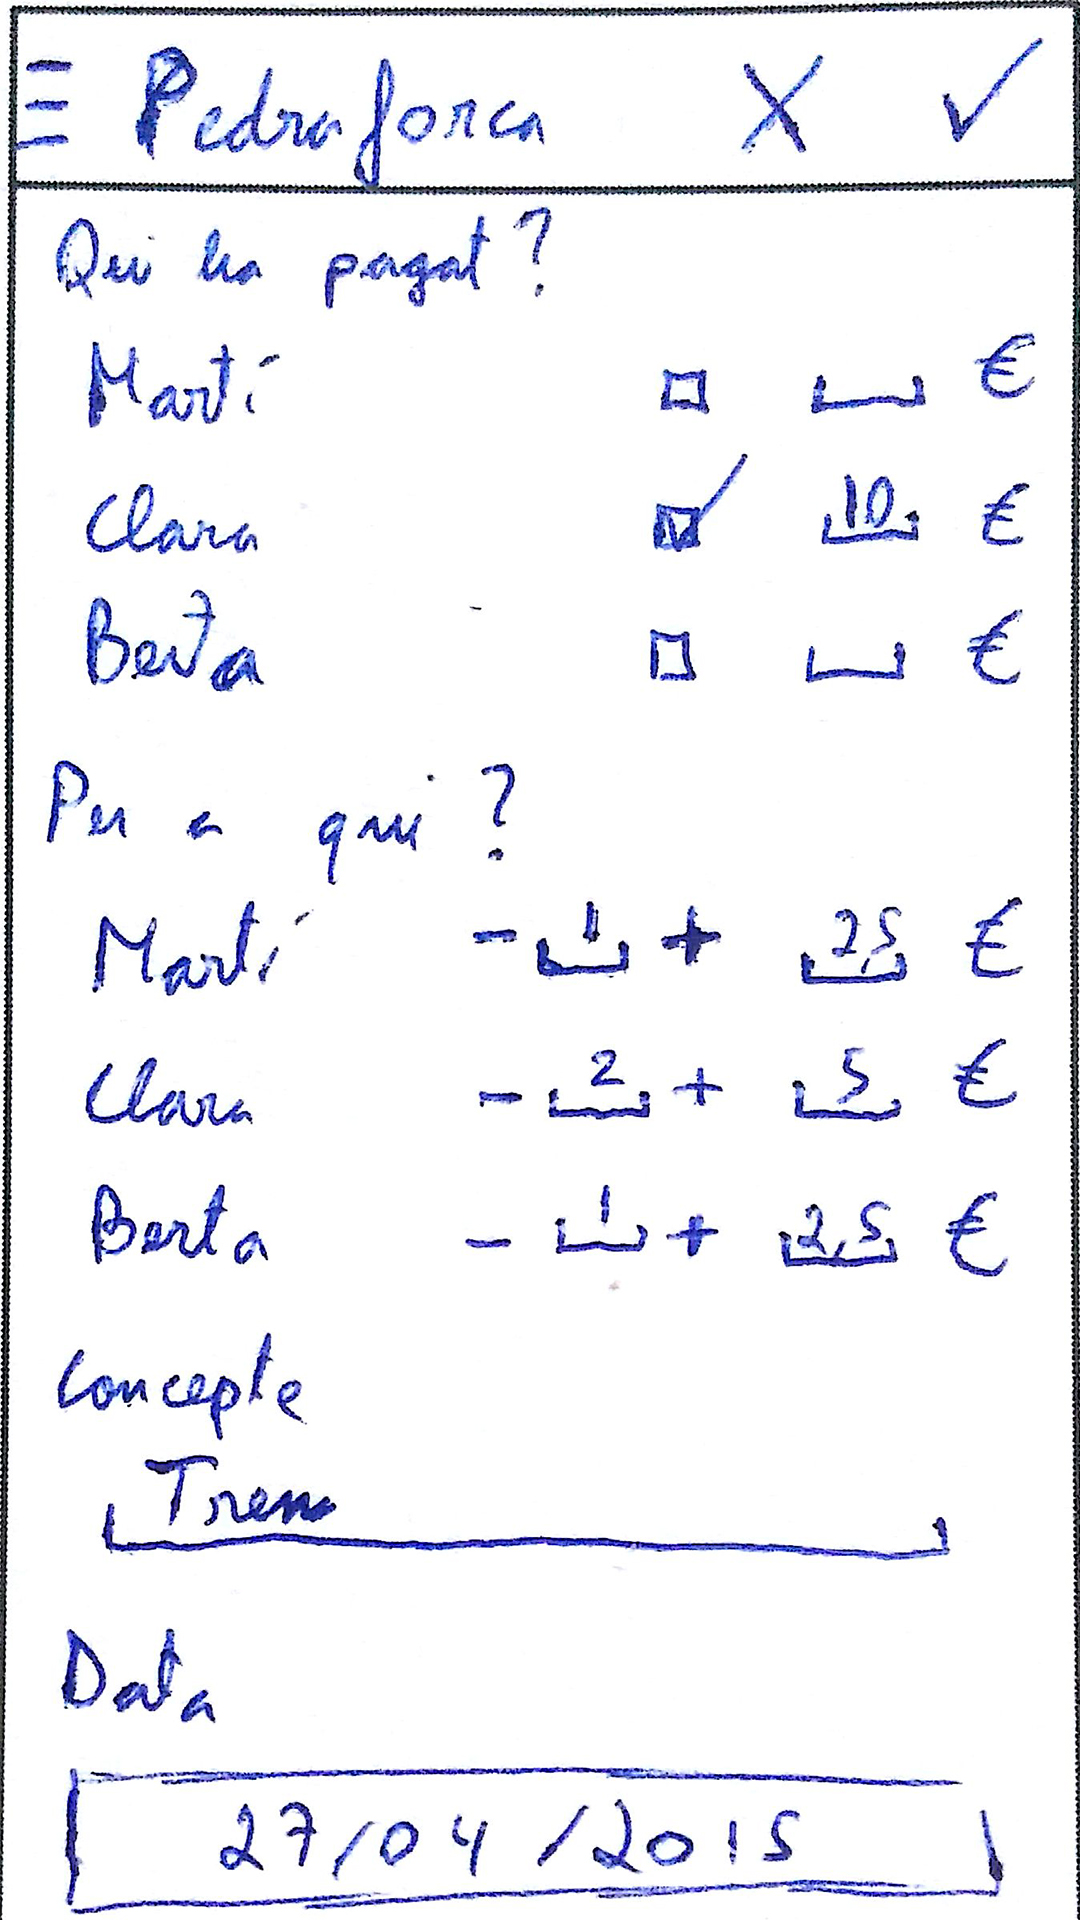
\includegraphics[width=50mm]{1_Add_group_transaction.jpg} &
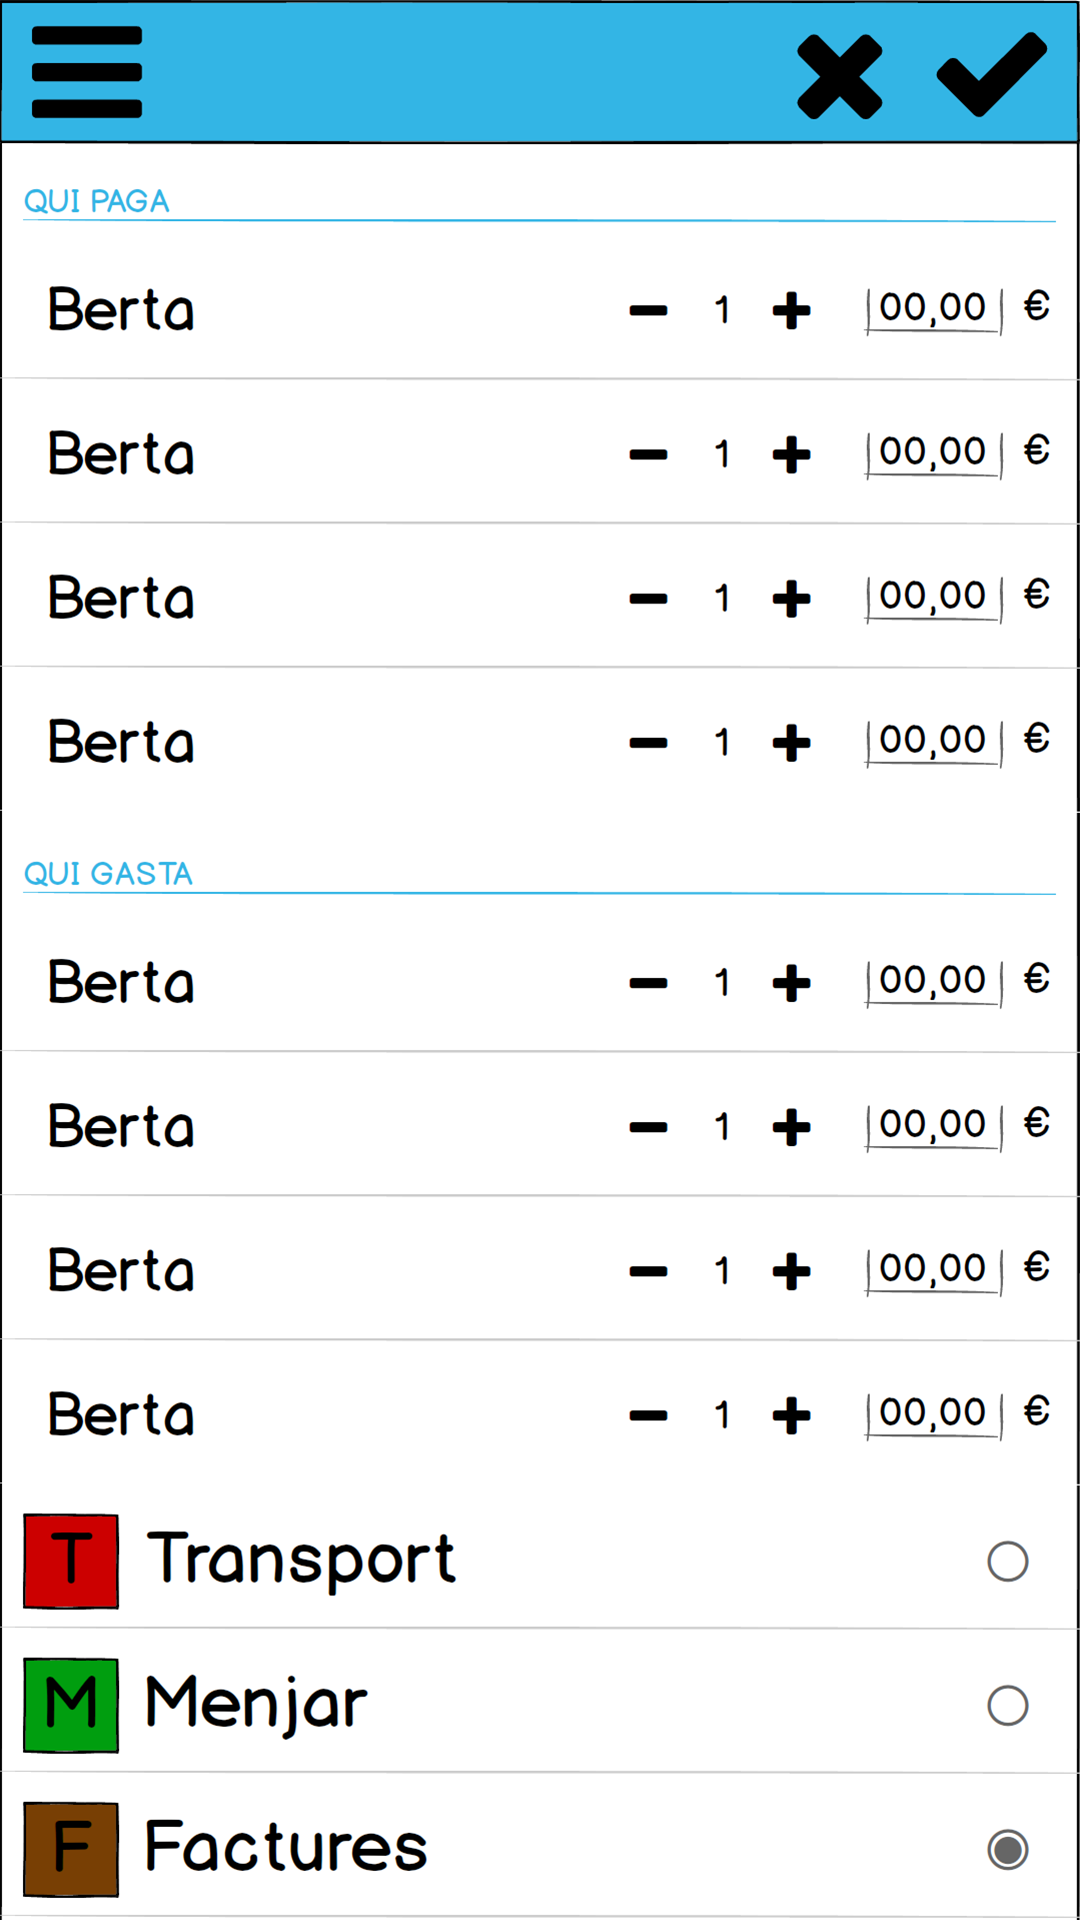
\includegraphics[width=50mm]{2_Add_group_transaction.png} &
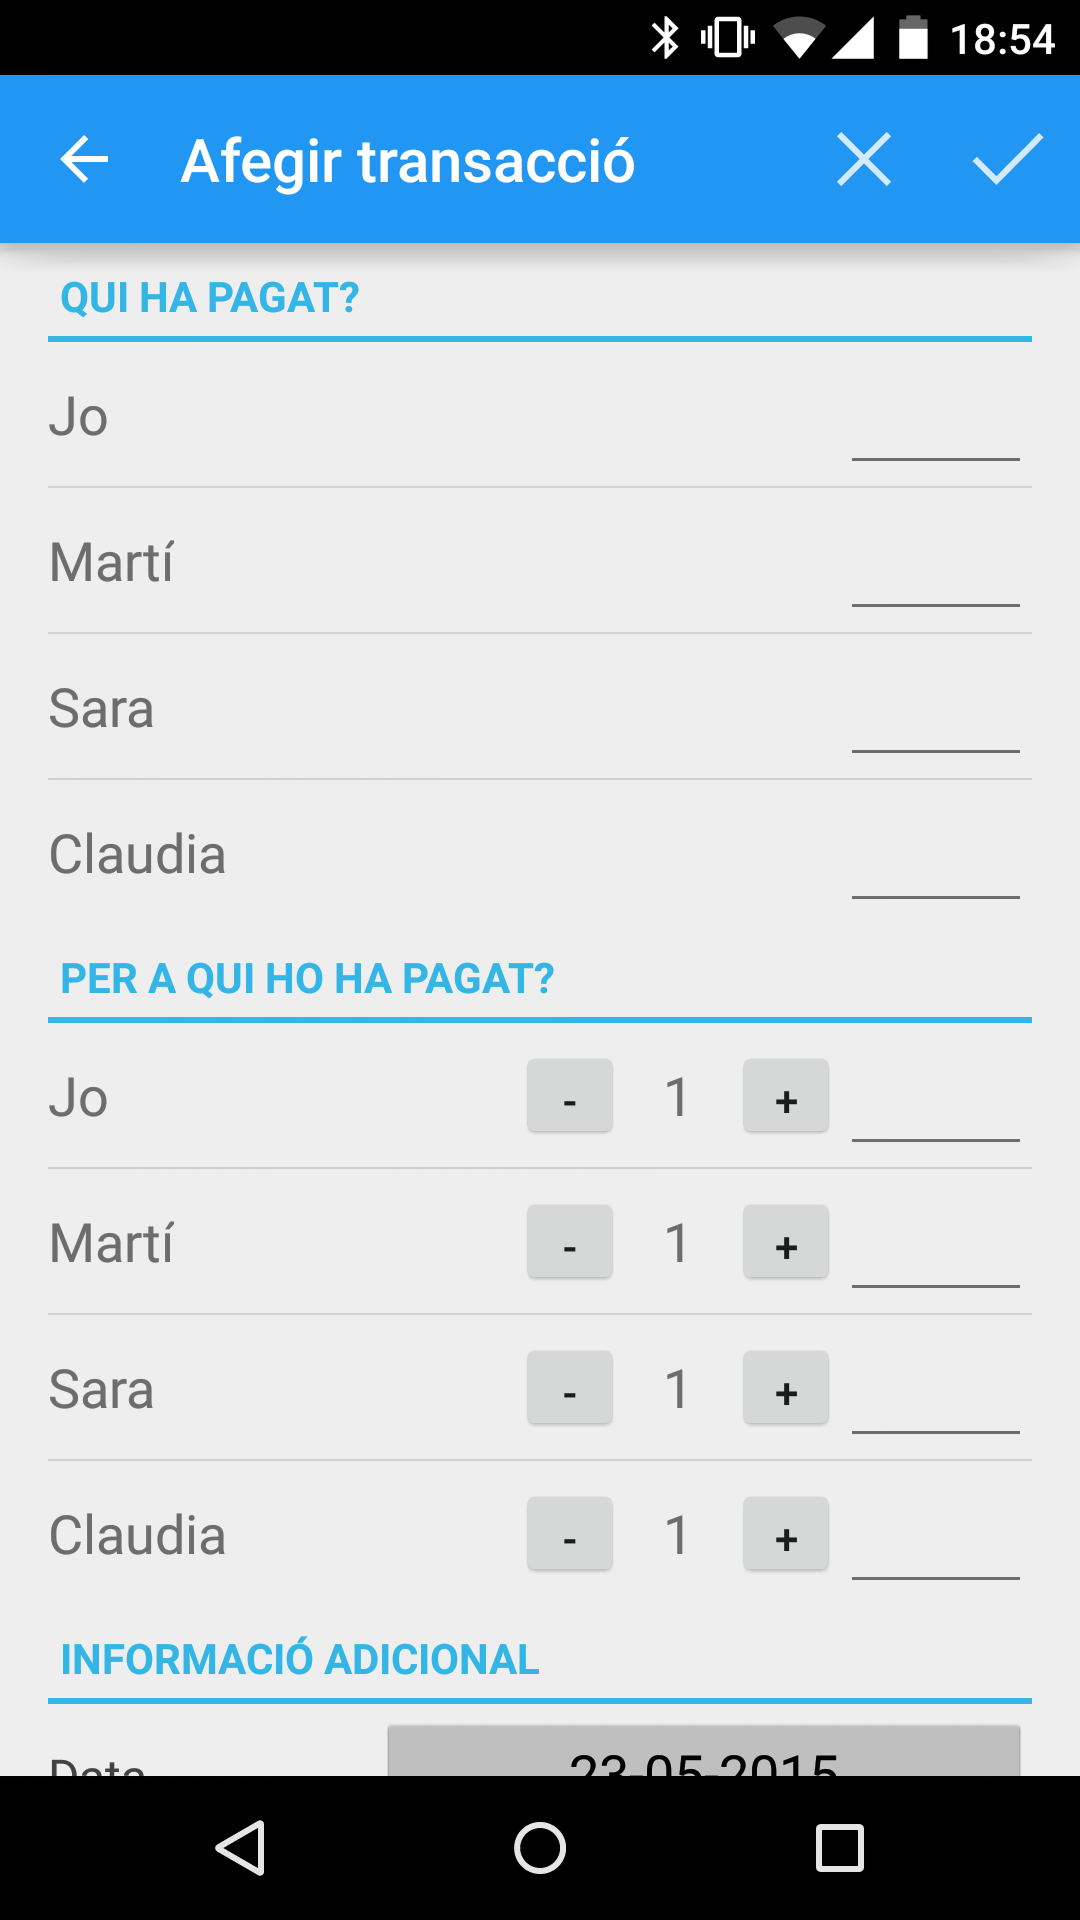
\includegraphics[width=50mm]{3_Add_group_transaction.png}  \\
\hline
Esbossos & Disseny Conceptual - intermedi & Disseny detallat - refinat \\
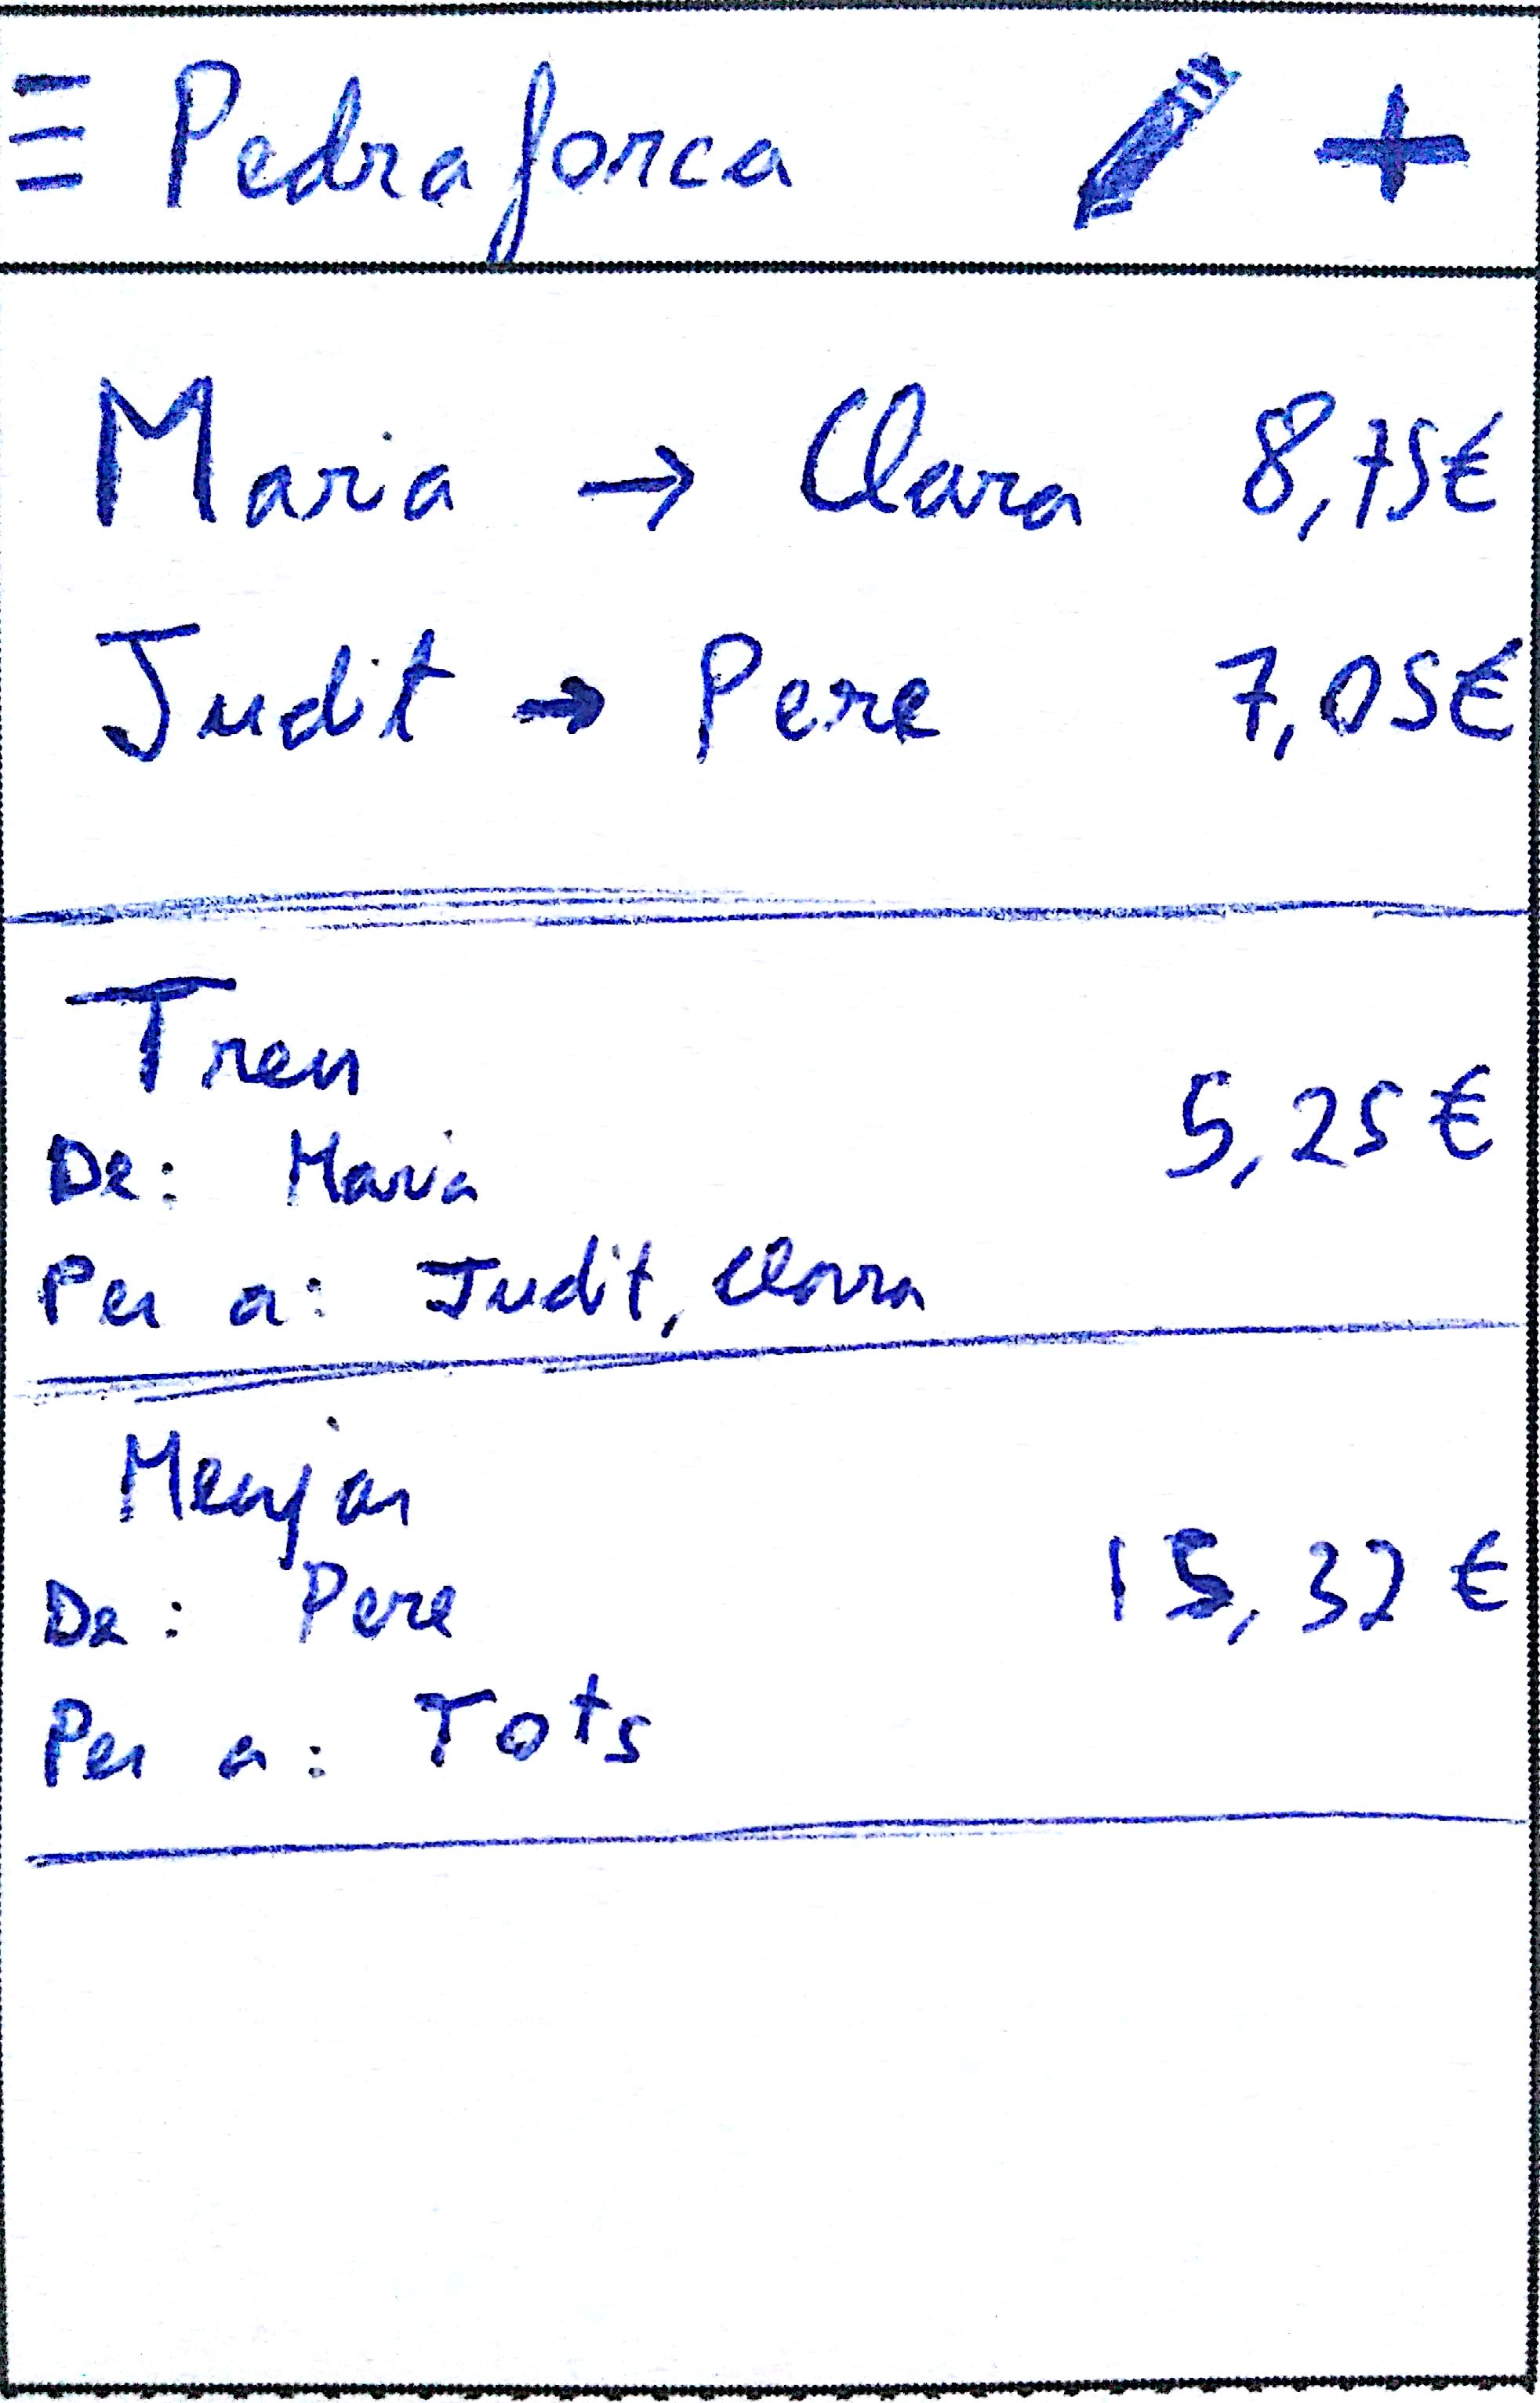
\includegraphics[width=50mm]{1_Group.jpg} &
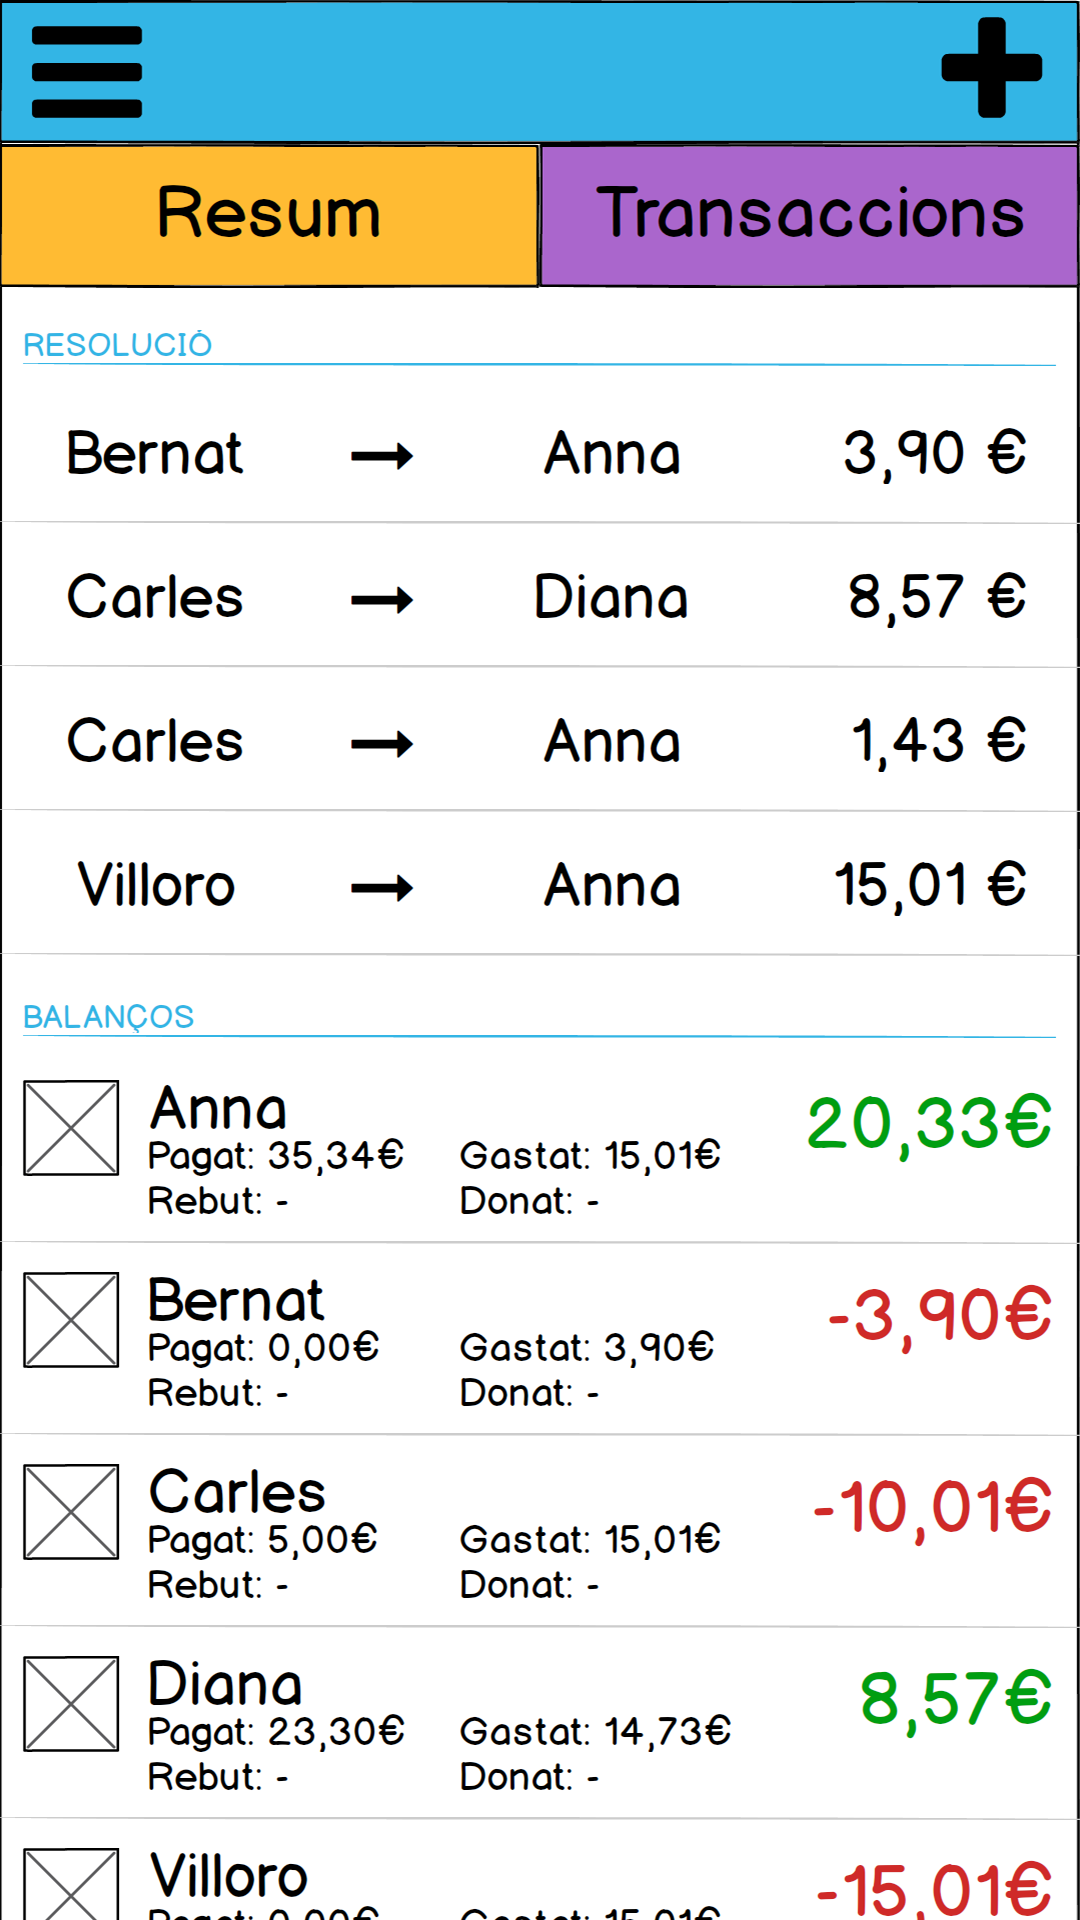
\includegraphics[width=50mm]{2_Group.png} &
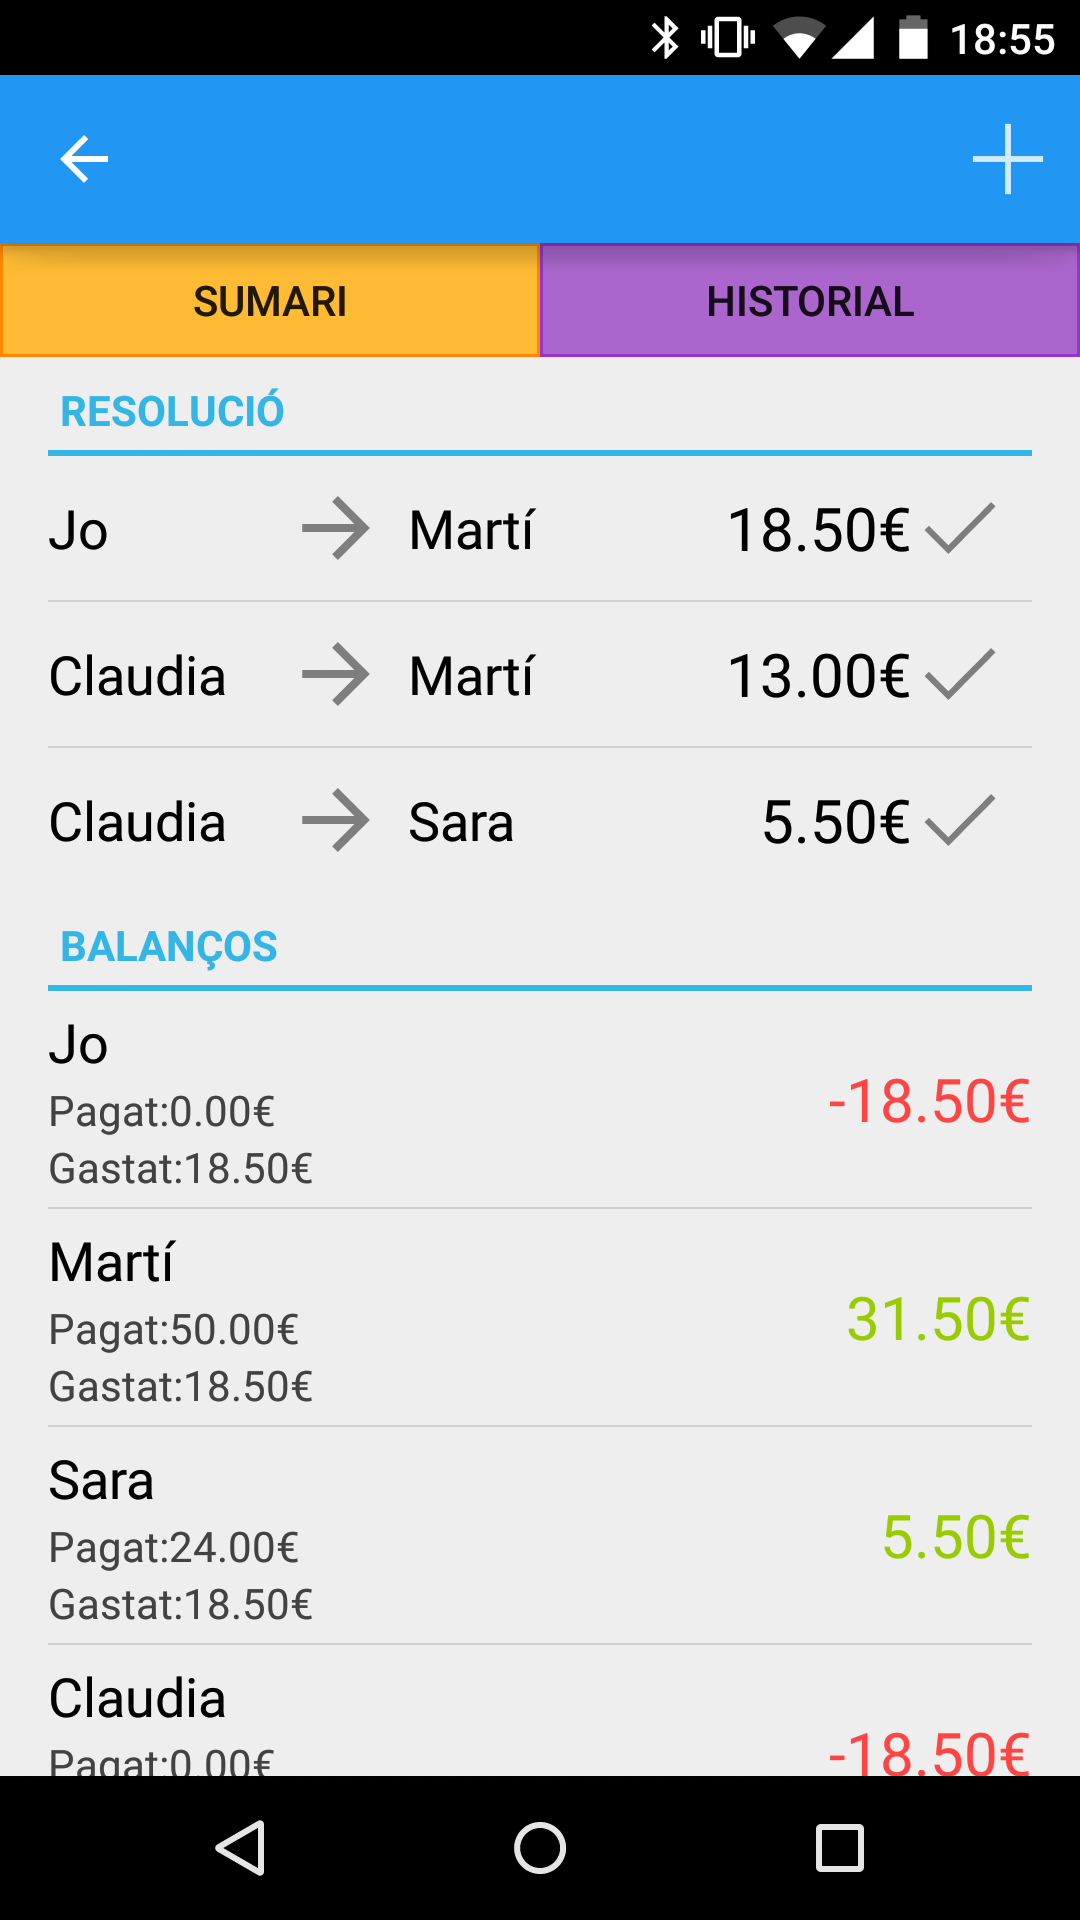
\includegraphics[width=50mm]{3_Group.png}  \\
\hline
\end{tabular}
\end{table}

\begin{table}
\caption{Imatges de l'aplicació a les diverses etapes del disseny 3}
\label{table:images_app3}
\begin{tabular}{| c | c | c |}
\hline
Esbossos & Disseny Conceptual - intermedi & Disseny detallat - refinat \\
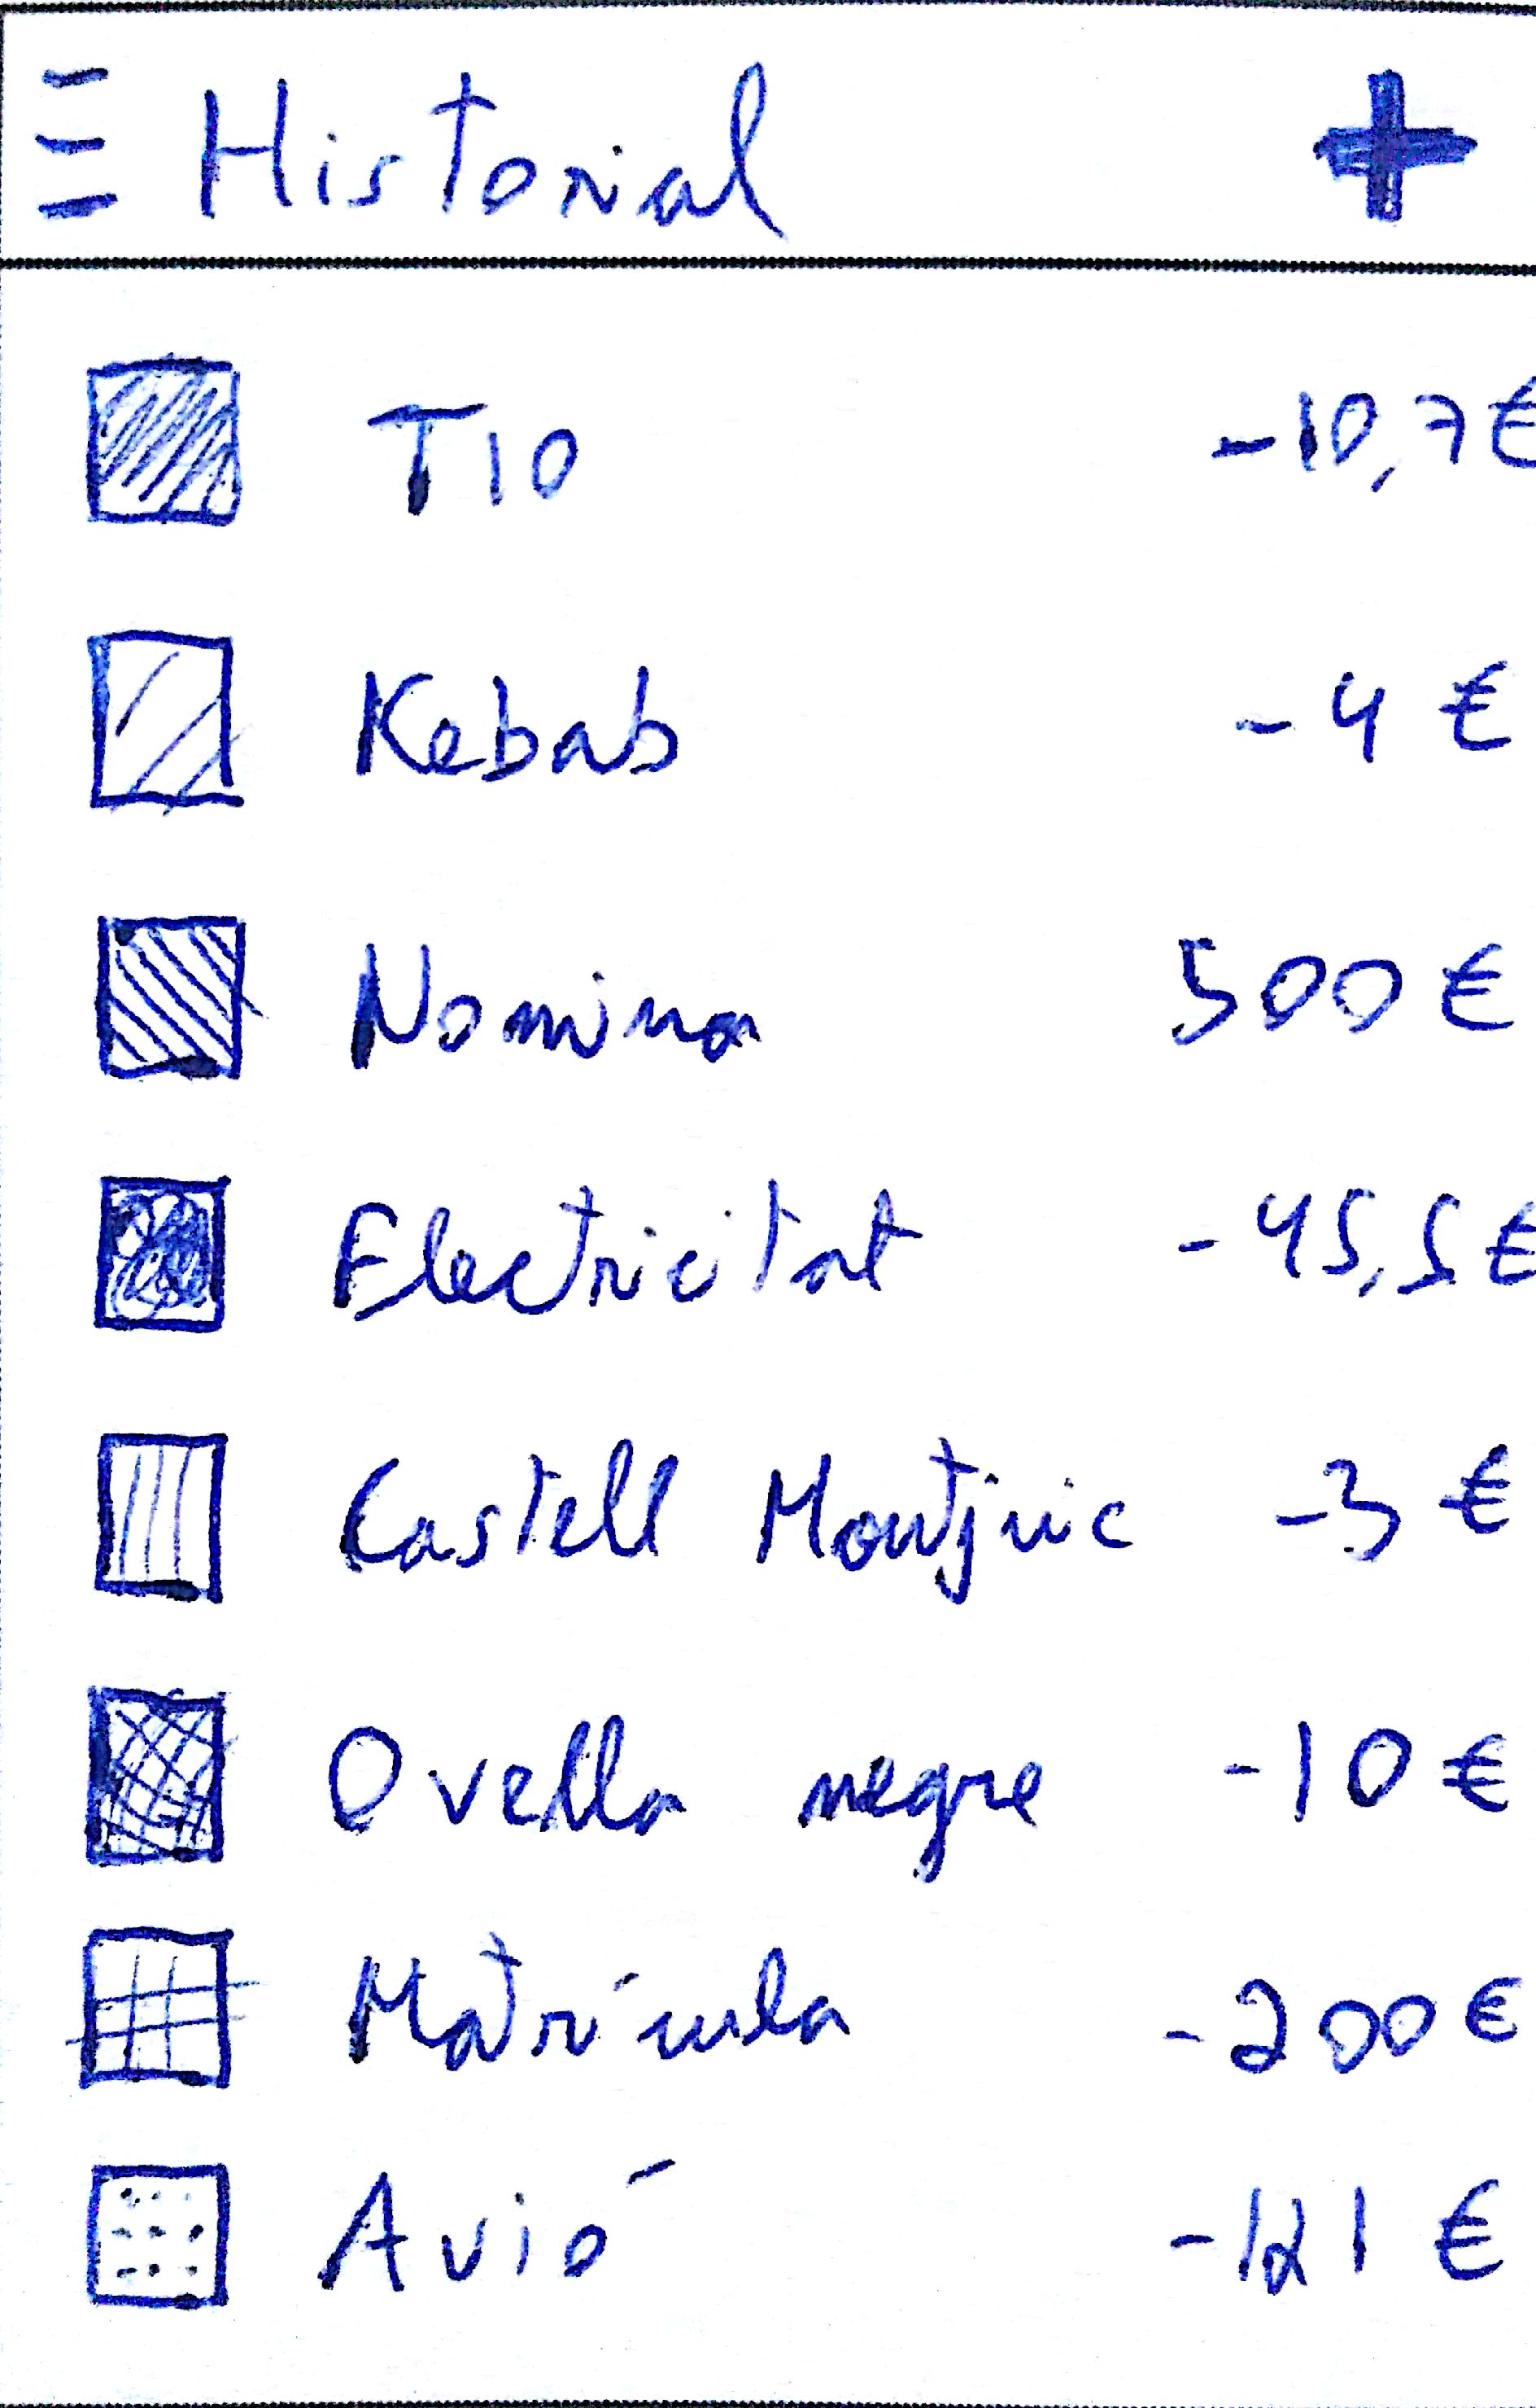
\includegraphics[width=50mm]{1_History.jpg} &
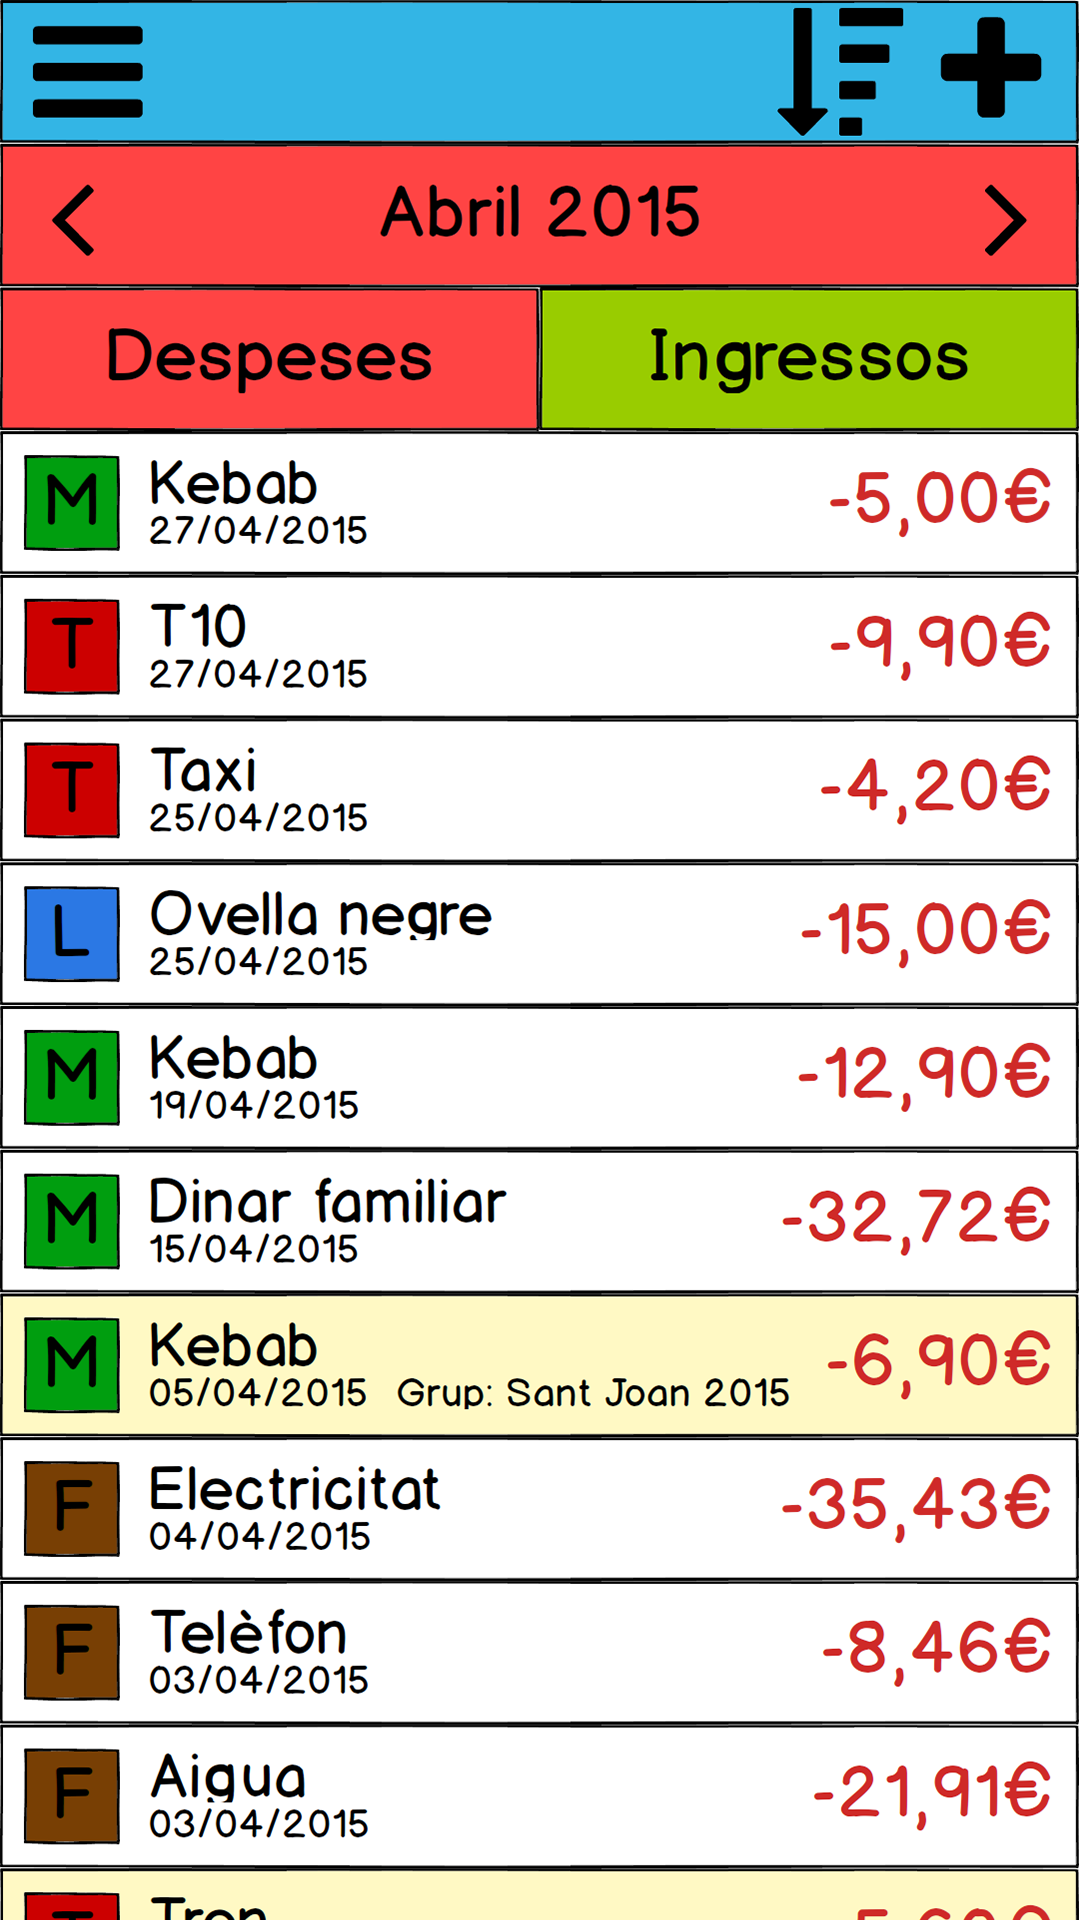
\includegraphics[width=50mm]{2_History.png} &
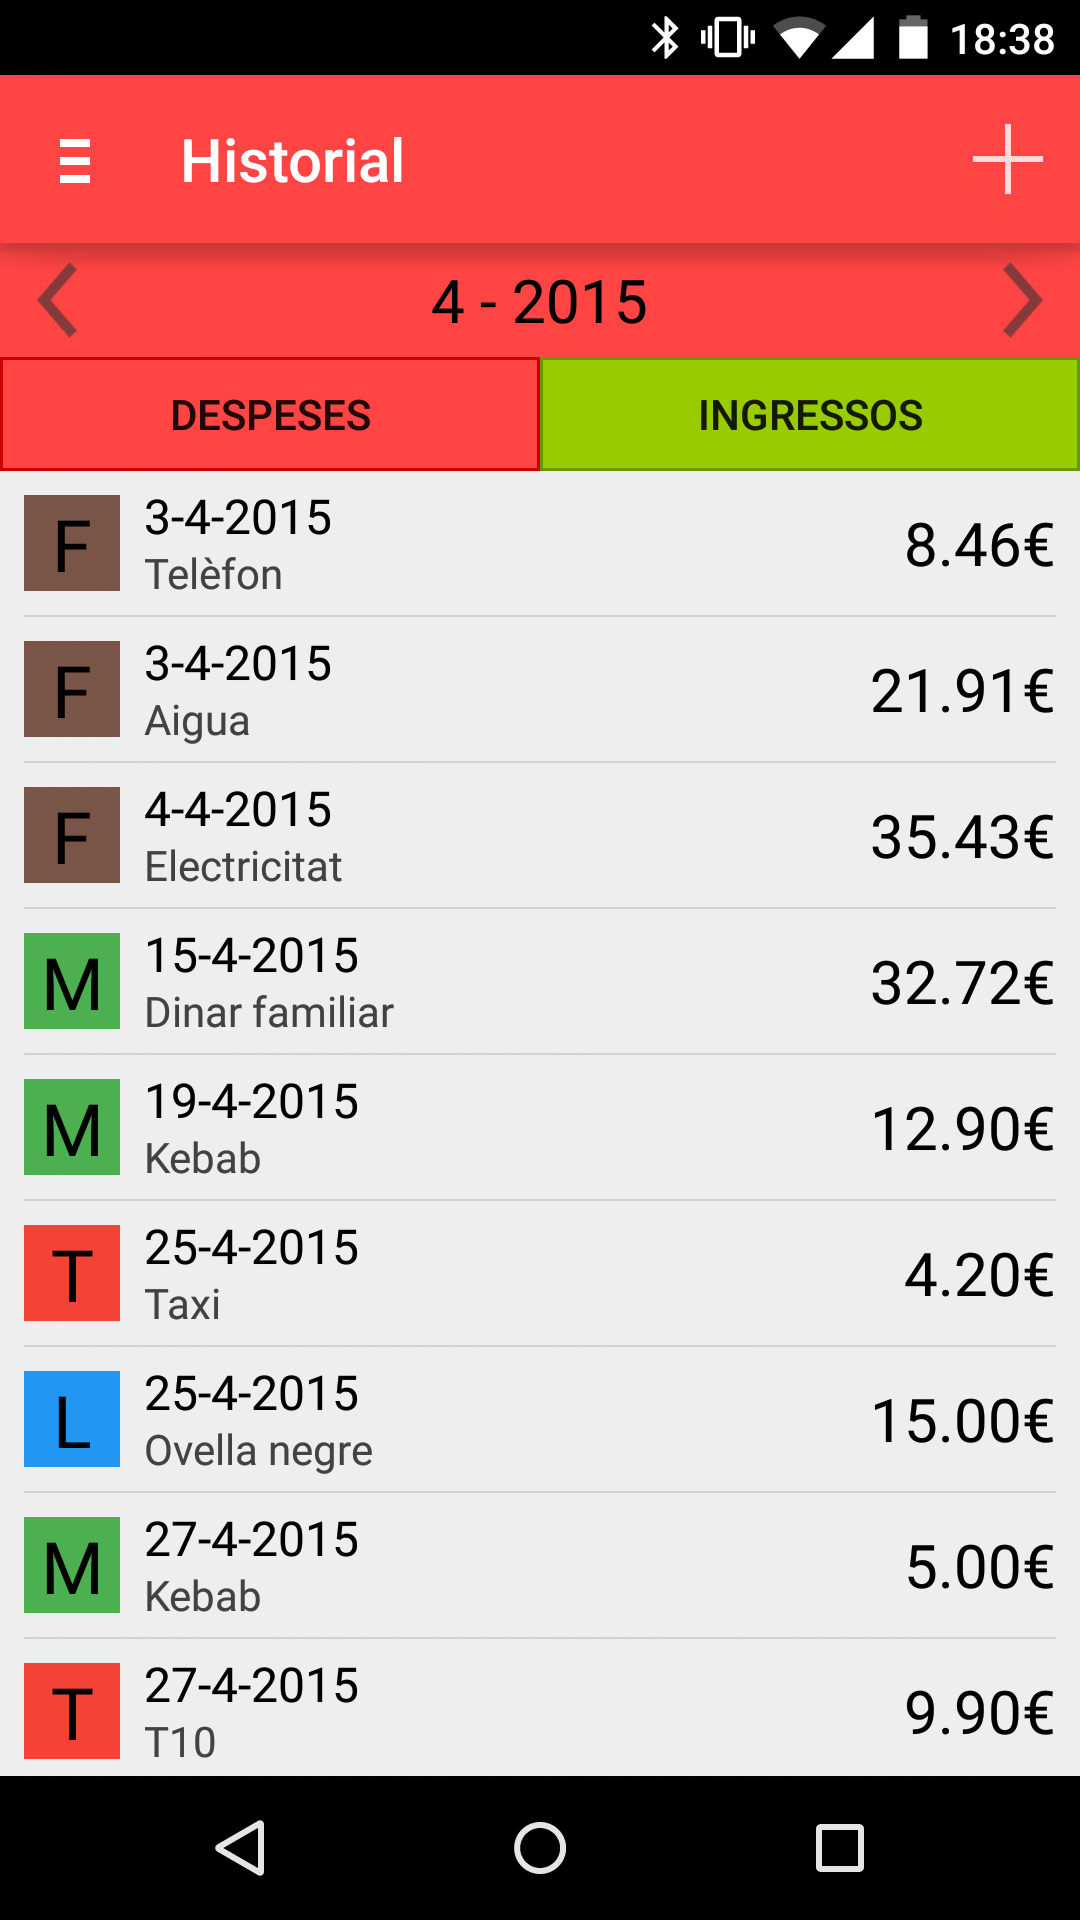
\includegraphics[width=50mm]{3_History.png}  \\
\hline
Esbossos & Disseny Conceptual - intermedi & Disseny detallat - refinat \\
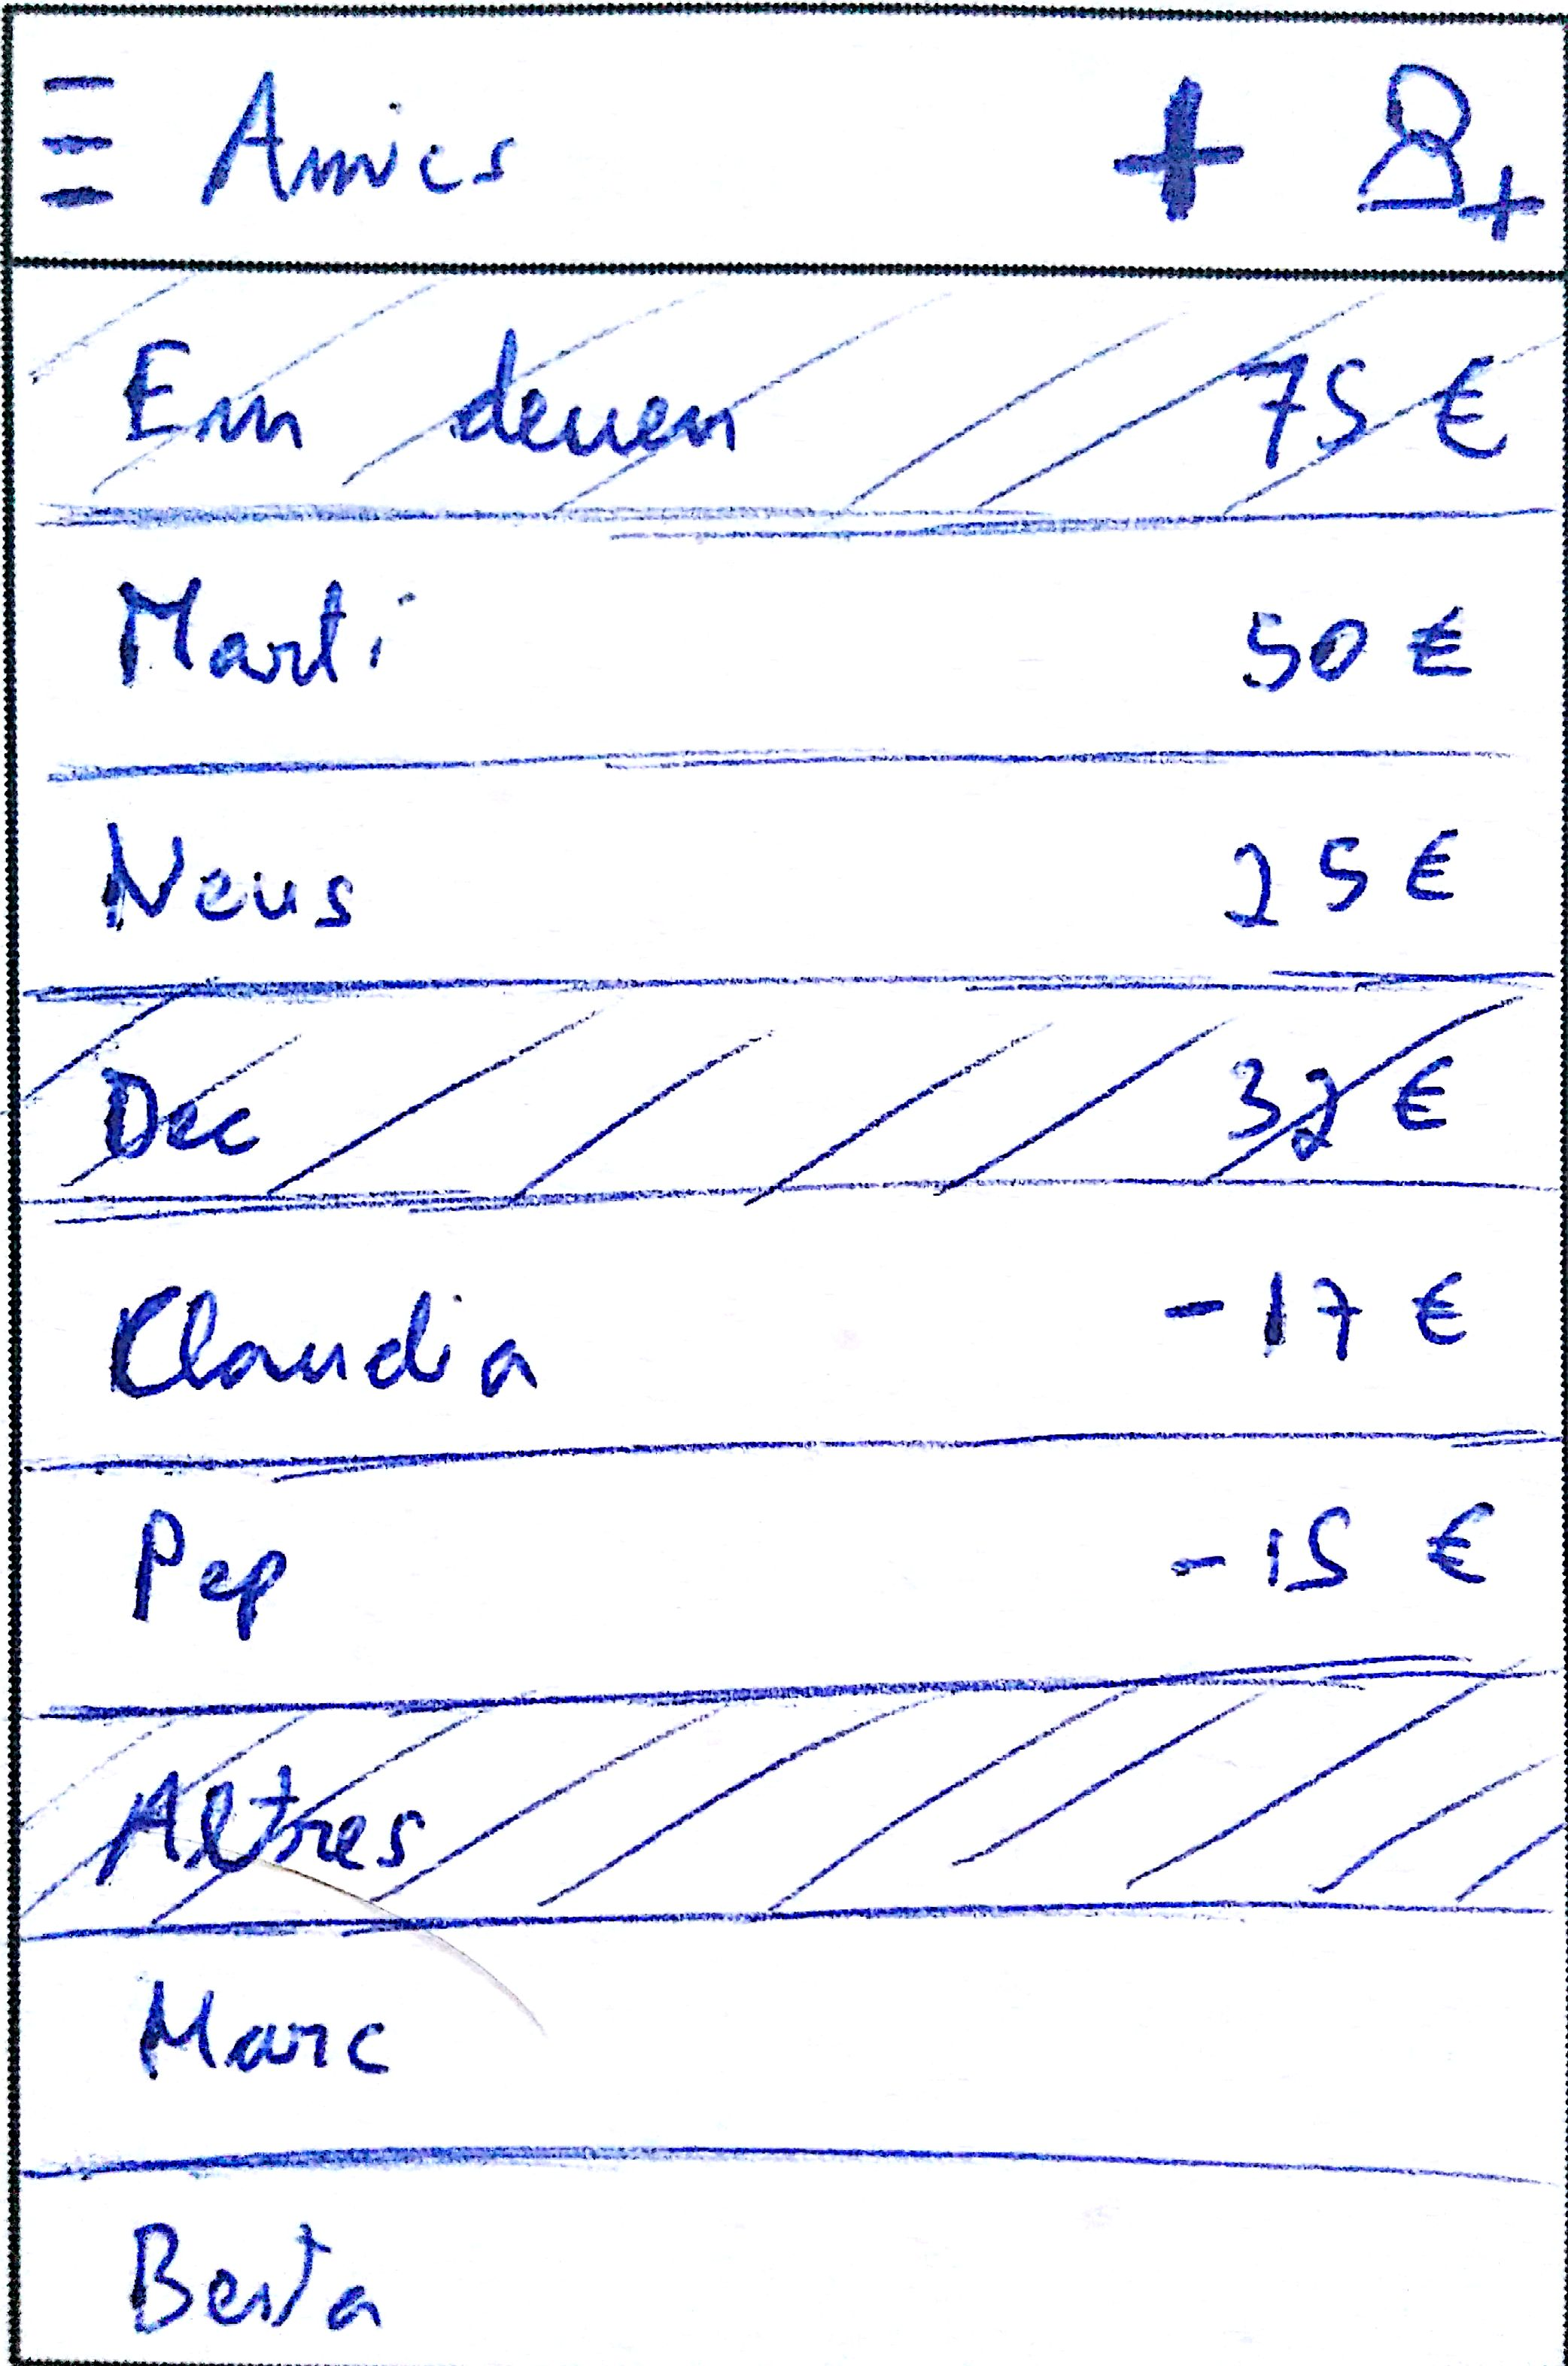
\includegraphics[width=50mm]{1_People.jpg} &
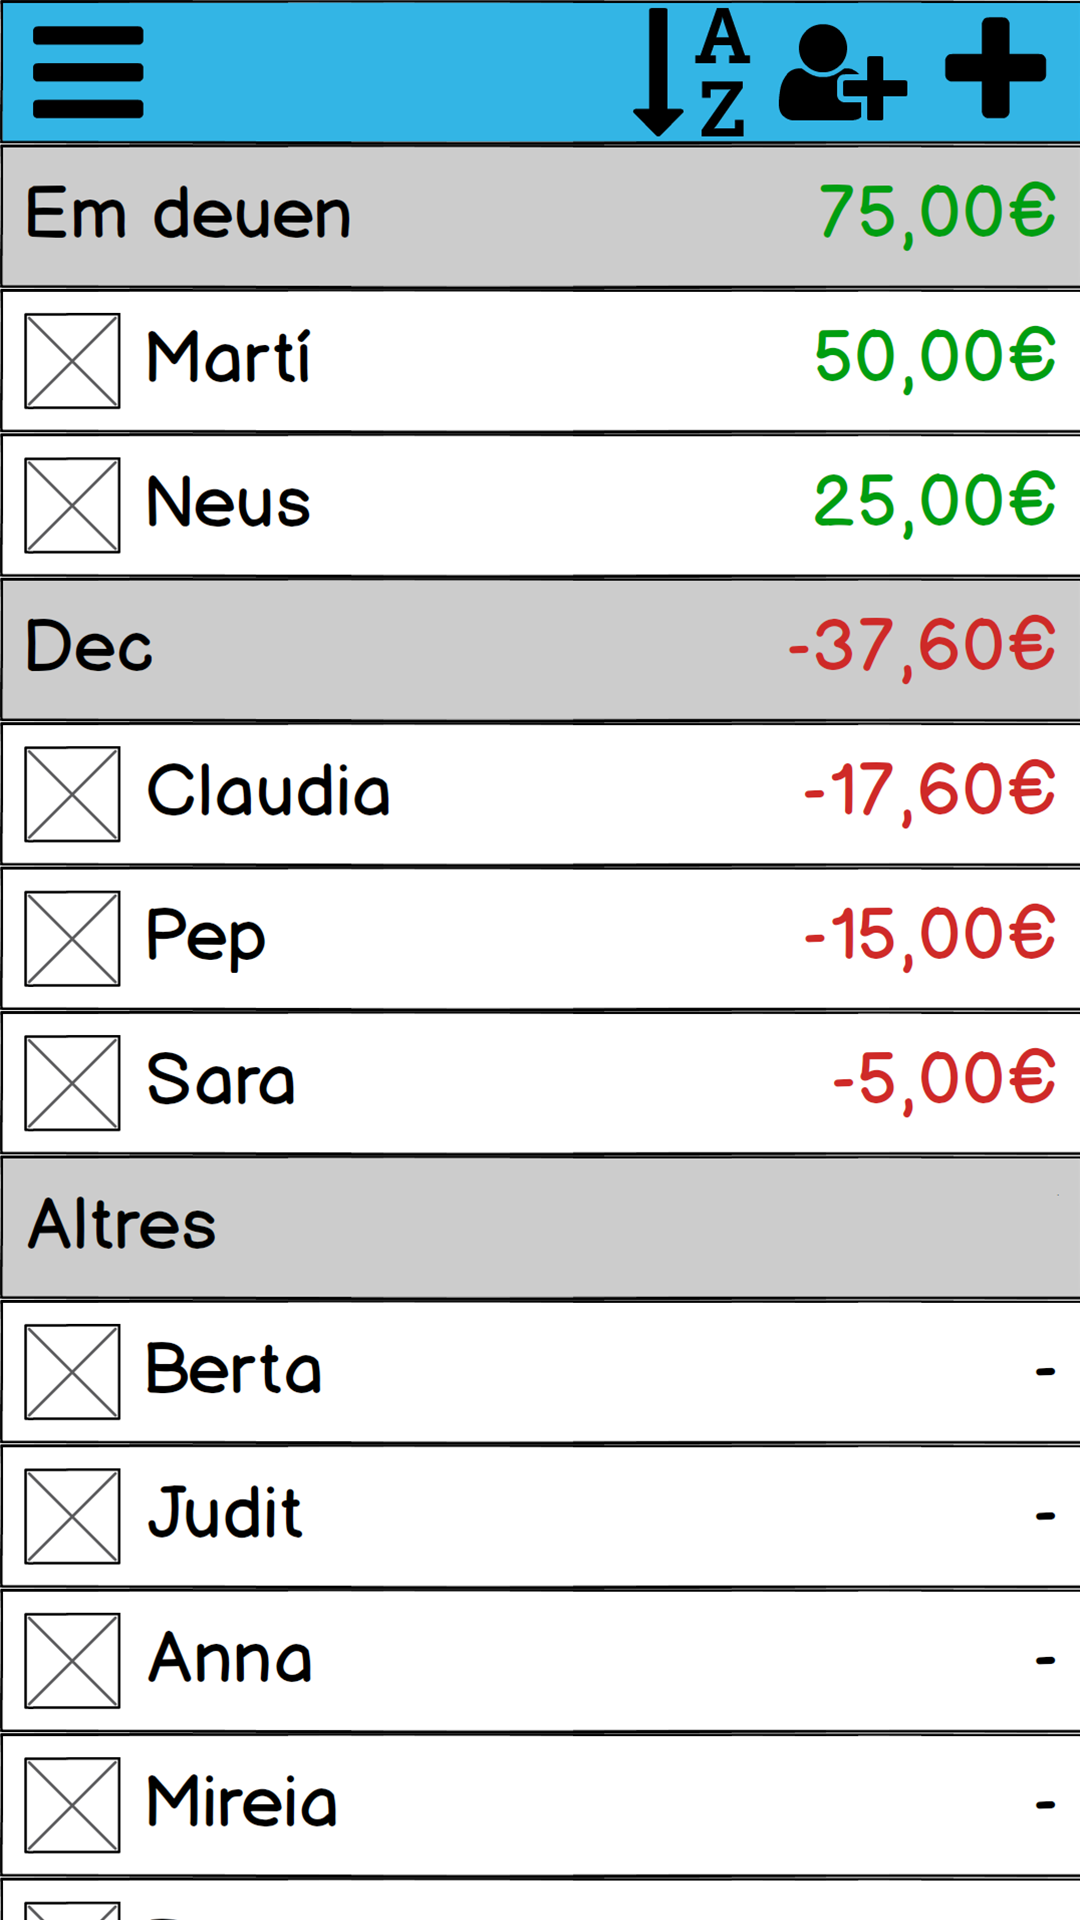
\includegraphics[width=50mm]{2_People.png} &
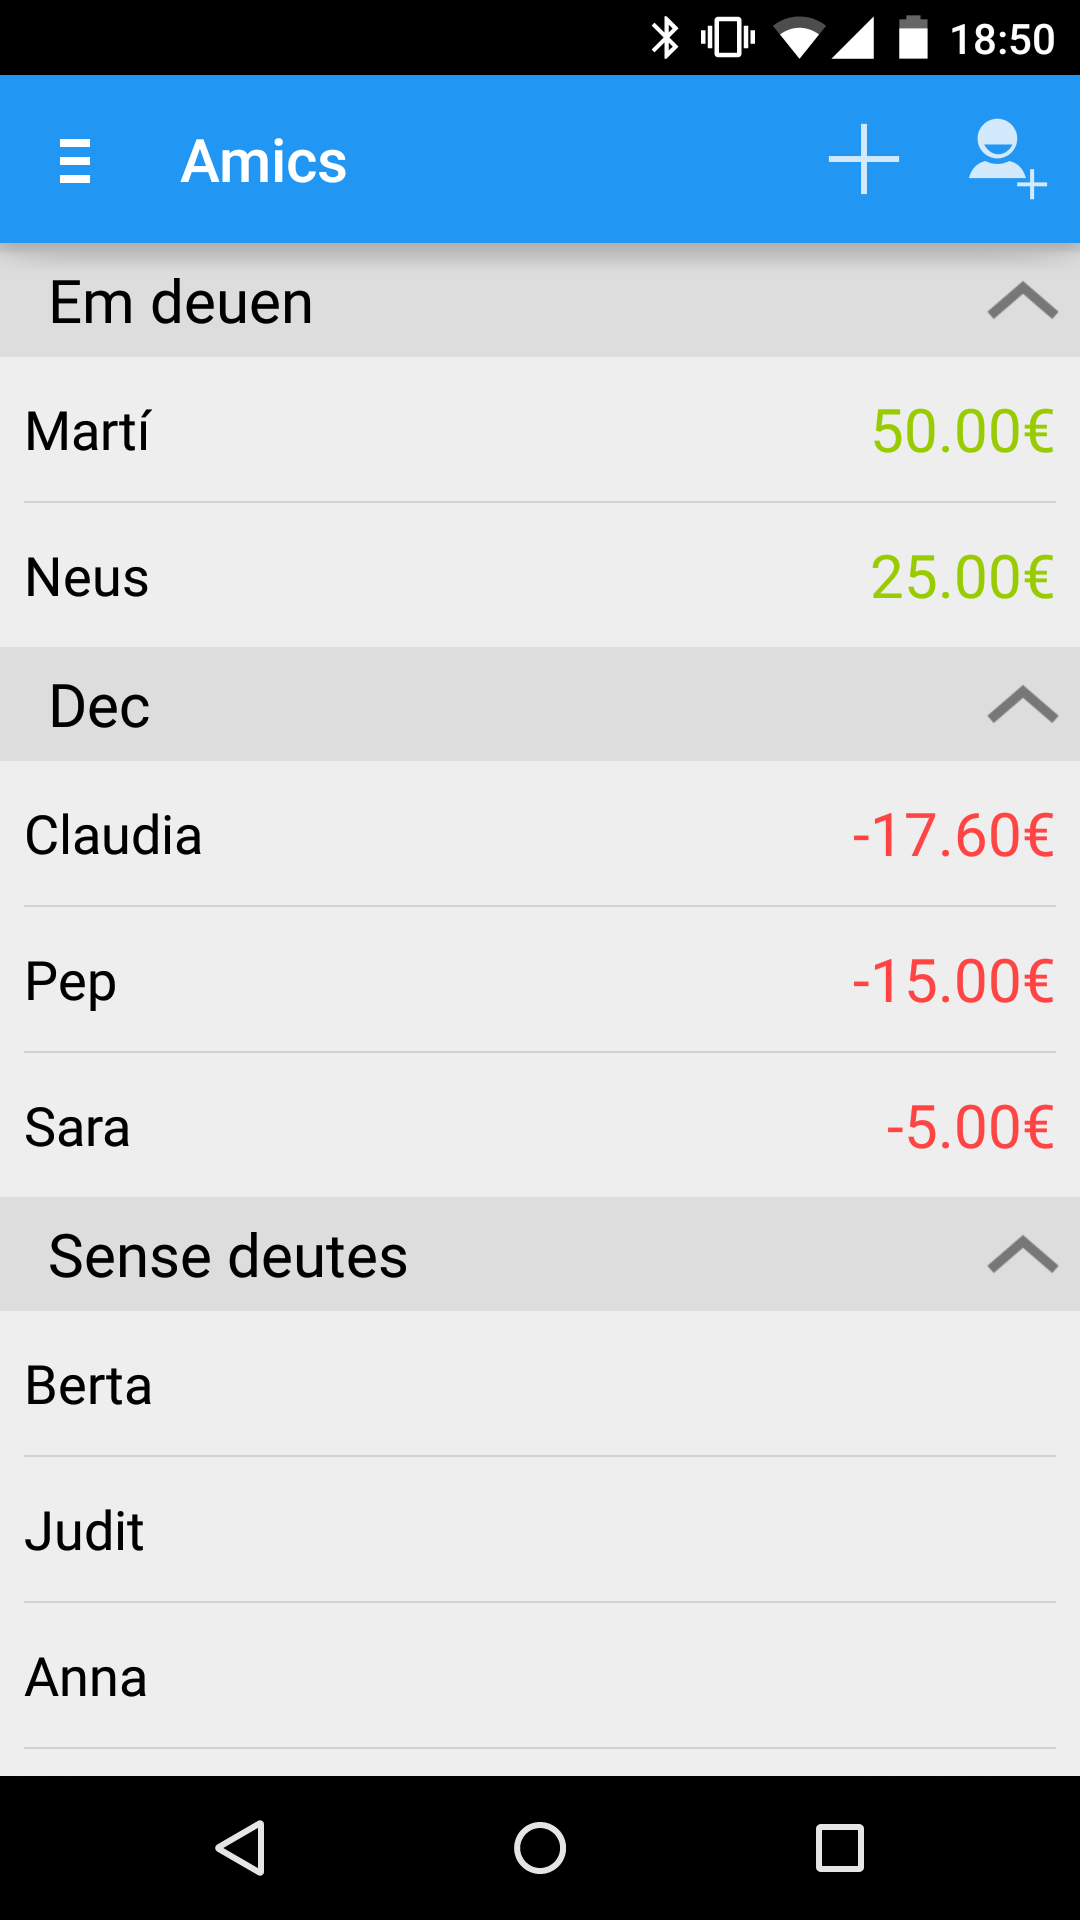
\includegraphics[width=50mm]{3_People.png}  \\
\hline
\end{tabular}
\end{table}

%TODO link a més imatges del disseny

\section{Implementació}
En aquesta etapa s'han creat prototips per conformar els dissenys de l'etapa anterior. A la taula \ref{table:prototypes} es poden veure els prototips que s'han creat. Els tres primers prototips venen a ser l'equivalent a prototips de paper, però enlloc de fer servir paper s'han fet servir dues aplicacions online que serveixen per fer prototips animats a partir d'imatges. Aquests es poden fer servir posteriorment en un \gls{smartphone} de manera que l'usuari té una experiència més propera a la realitat.

En quan als prototips en si, en primer lloc s'ha fet un prototip horitzontal de baixa fidelitat (PH1) per una primera presa de contacte amb el producte previst amb una fidelitat baixa. Després s'han creat 3 prototips de mitja fidelitat. El primer (PH2) és un prototip horitzontal que ha servit per definir la navegació en línies generals. El segon (PV1) és un prototip vertical que ha servit per explorar dues possibilitats que hi havien a l'hora de tractar els ingressos i les despeses. El tercer (PL1) és un prototip local programat per a comprovar si els usuaris es sentien còmodes amb la pantalla d'afegir una transacció grupal. Finalment s'ha fet un prototip d'alta fidelitat, amb les seccions i funcions més importants, el qual és molt pròxim a com ha de ser l'aplicació a la realitat. 

\begin{table}
\caption{Prototips creats}
\label{table:prototypes}
\begin{tabular}{ | p{1.6cm} | c | p{1.9cm} | l | l |}
\hline
\textbf{Codi} & \textbf{Icona} & \textbf{Tipus de Prototip} & \textbf{Fidelitat} & \textbf{URL}\\ 
\hline
PH1 & 
\includegraphics[width=0.7cm]{PH1.png} & Horitzontal & Baixa & \href{http://invis.io/3F2TDUWP8}{http://invis.io/3F2TDUWP8} \\
\hline
PH2 & 
\includegraphics[width=0.7cm]{PH2.png} & Horitzontal & Mitja & \href{https://www.flinto.com/p/72ad65cd}{https://www.flinto.com/p/72ad65cd} \\
\hline
PV1 & 
\includegraphics[width=0.7cm]{PV1.png} & Vertical & Mitja & \href{https://www.flinto.com/p/fee8156d}{https://www.flinto.com/p/fee8156d} \\
\hline
PL1 & 
\includegraphics[width=0.7cm]{PL1.png} & Local & Mitja &  \\ %TODO link
\hline
Expensor beta & 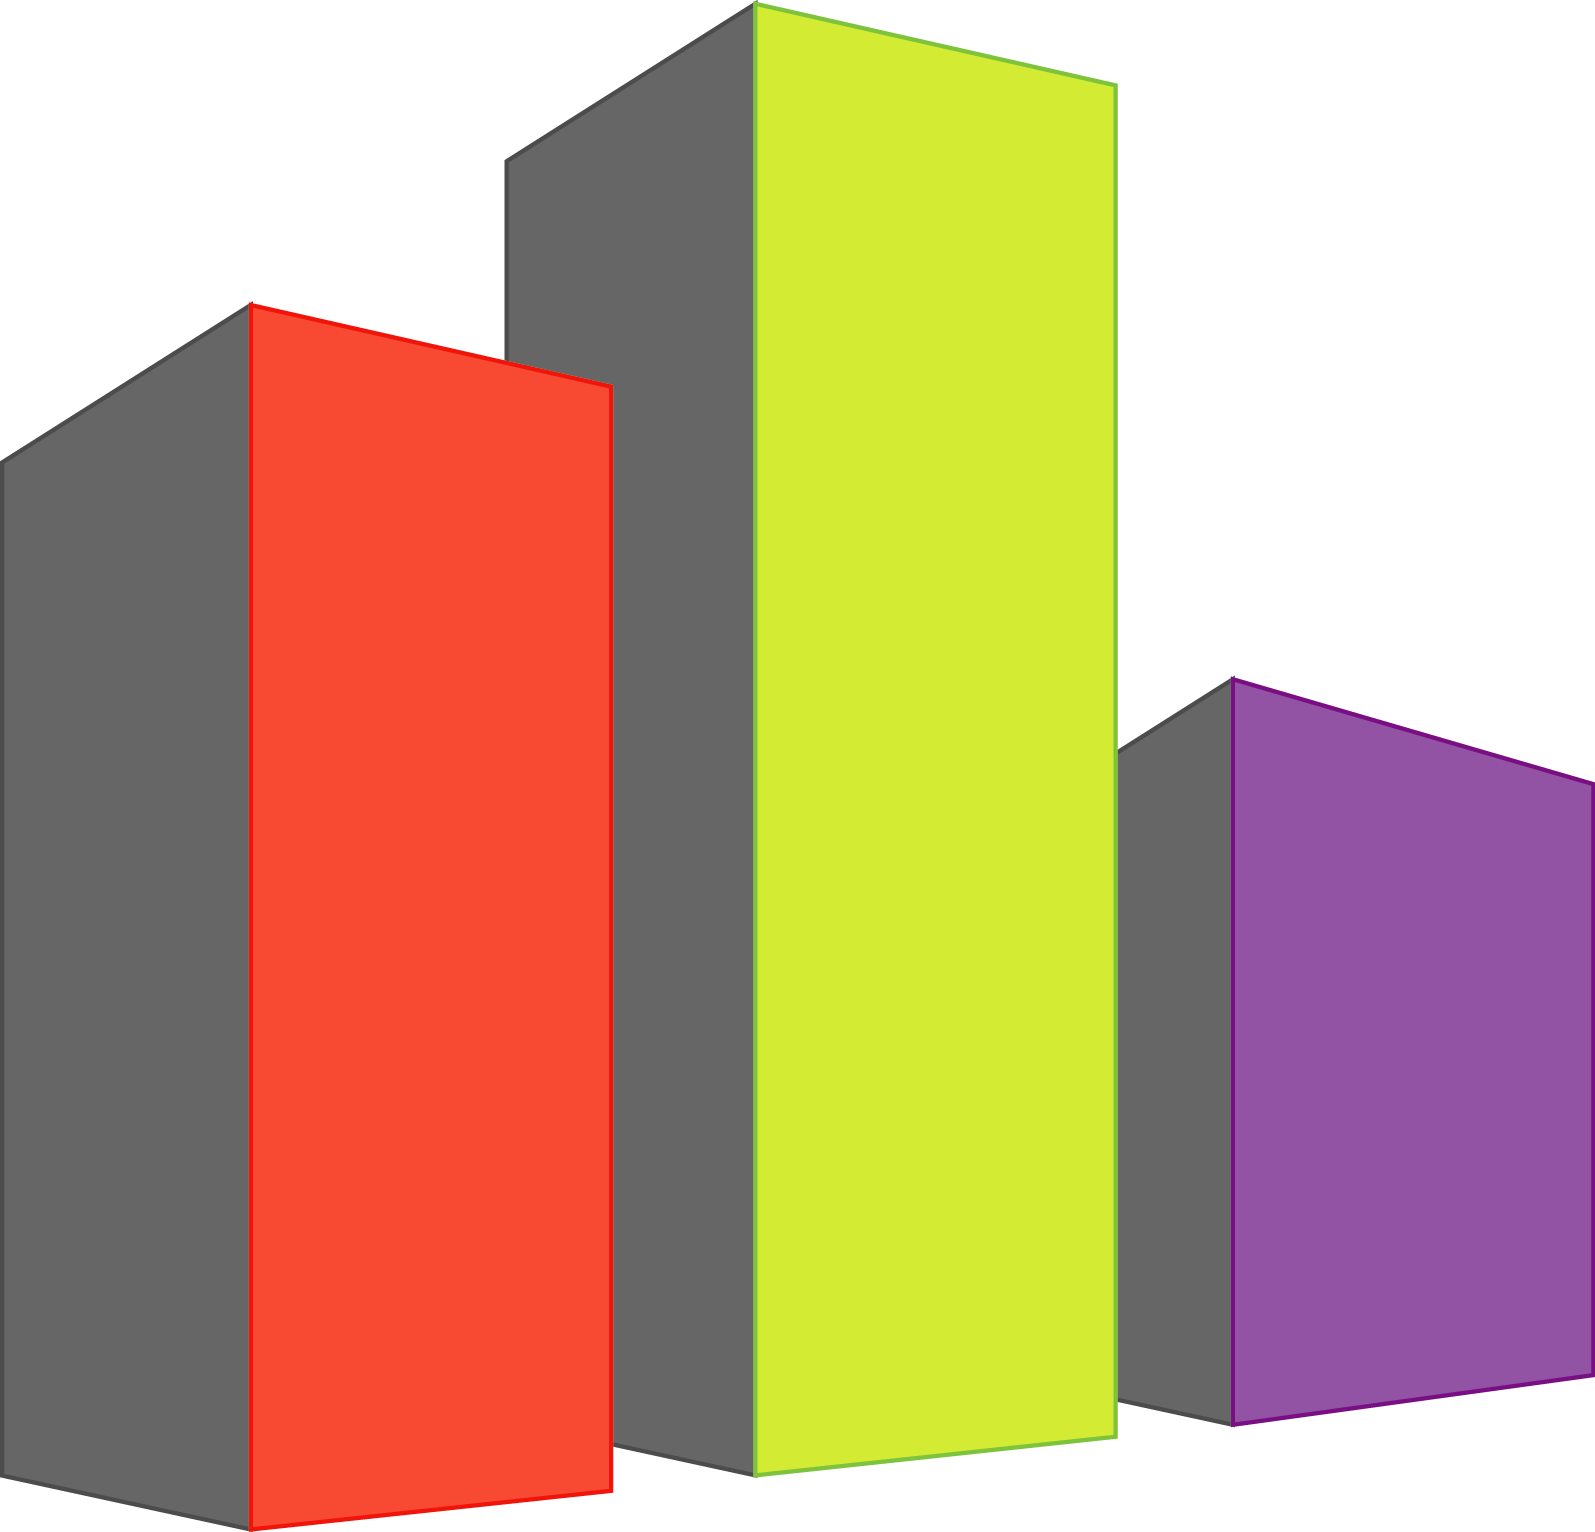
\includegraphics[width=0.7cm]{logo.png} & Complet & Alta &  \\ %TODO link
\hline
\end{tabular}
\end{table}

\section{Avaluació}
En aquesta etapa l'objectiu era validar, mitjançant els diversos prototips, que els dissenys creats garantien una bona \ac{UX}. A les primeres iteracions de l'estudi, quan els prototips i els dissenys eren de baixa fidelitat, aquests només s'han mostrat a un grup molt reduït d'usuaris de confiança. I és que no tots els usuaris entenen amb facilitat dissenys de baixa fidelitat.

\subsubsection{Avaluació formativa}
Un cop es treballava amb prototips de fidelitat mitja (PH2, PV1 i PL1), s'han concertat entrevistes amb els diferents usuaris per a que els provessin. Aquestes entrevistes s'han fet seguint una plantilla (figura \ref{fig:qf}) per fer una avaluació formativa als prototips. En total s'ha fet 22 entrevistes. %TODO link entrevistes
És important comentar que els prototips de mitja fidelitat s'han anat millorant, quan ha estat possible, a mesura que els usuaris aportaven la seva opinió en forma d'avaluació formativa. És per això que si es llegeixen les entrevistes i es miren els prototips, hi ha comentaris dels usuaris que sembla que no tinguin sentit, perquè s'ha tingut en compte i millorat el prototip en qüestió conseqüentment. 

\begin{figure}[htp]
\centering
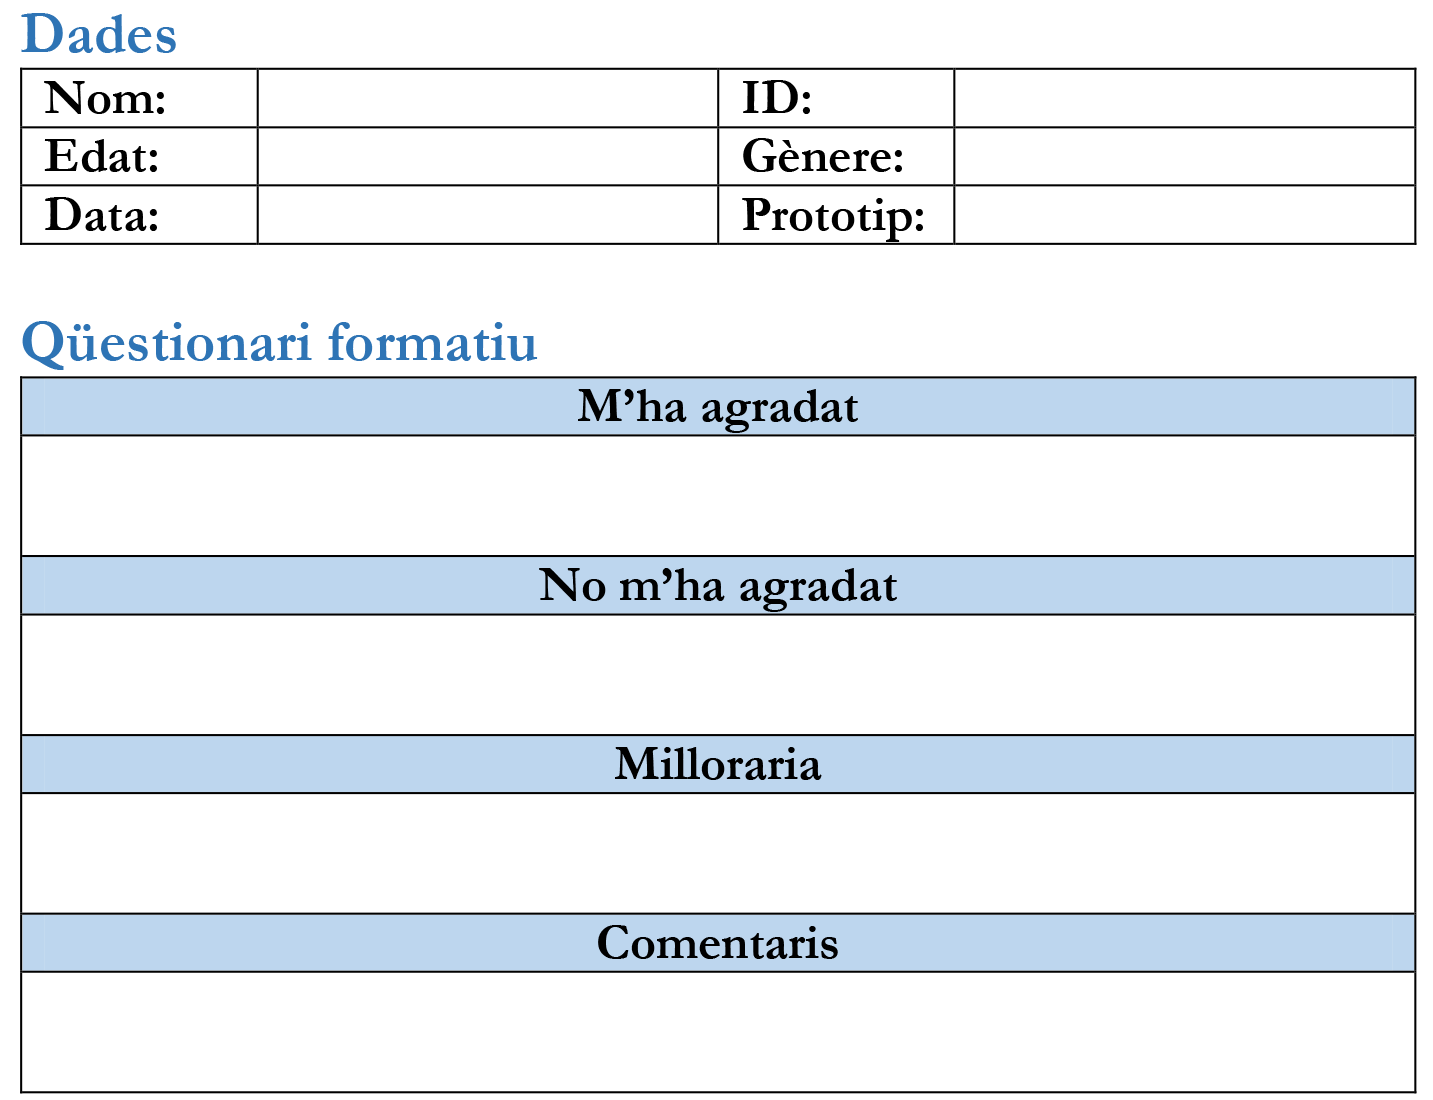
\includegraphics[scale=1]{qf.png}
\caption{Plantilla per a l'avaluació formativa}\label{fig:qf}
\end{figure}

\subsubsection{Avaluació sumarial 1}
Després de l'avaluació formativa s'ha passat a fer l'avaluació sumarial de l'aplicació. S'ha fet en dues parts, una primera avaluant  el prototip final (Expensor beta) juntament amb les 10 aplicacions ja existents. A la segona part s'ha avaluat amb més detall les 2 aplicacions de l'etapa anterior juntament amb el prototip final.

Aquesta primera part de l'avaluació sumarial s'ha fet deixant provar les aplicacions a 4 usuaris i després demanant-los que omplissin el qüestionari SUS. S'ha fet servir aquest qüestionari perquè és ràpid de fer, només té 10 preguntes, i permet fer un primer anàlisi de fins a quin punt cada aplicació garanteix una bona \ac{UX} o no. A la figura \ref{fig:SUS_analisi} es pot veure la puntuació (mitjana dels 4 usuaris) del qüestionari SUS per a cada aplicació. Els valors del qüestionari SUS estan entre 0 i 100, on el 100 és la millor puntuació possible. A més a la figura \ref{fig:SUS_table} es pot veure el resultat mitja de cada pregunta per cada aplicació (els valors estan entre 0 i 10).

\begin{figure}[htp]
\centering
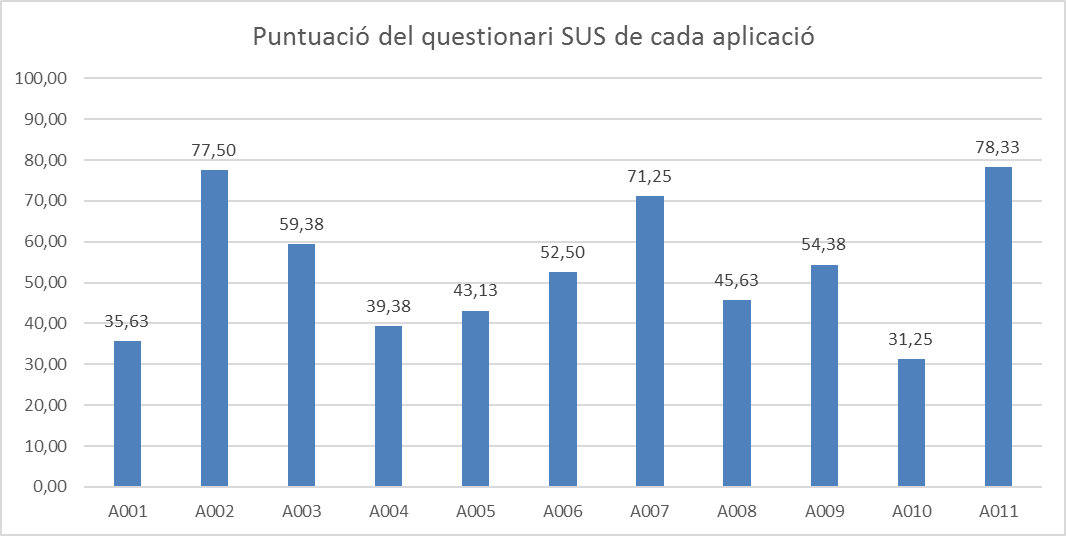
\includegraphics[scale=0.8]{SUS_analisi_1.png}
\caption{Resultats del questionari SUS per cada aplicació}\label{fig:SUS_analisi}
\end{figure}

\begin{figure}[htp]
\centering
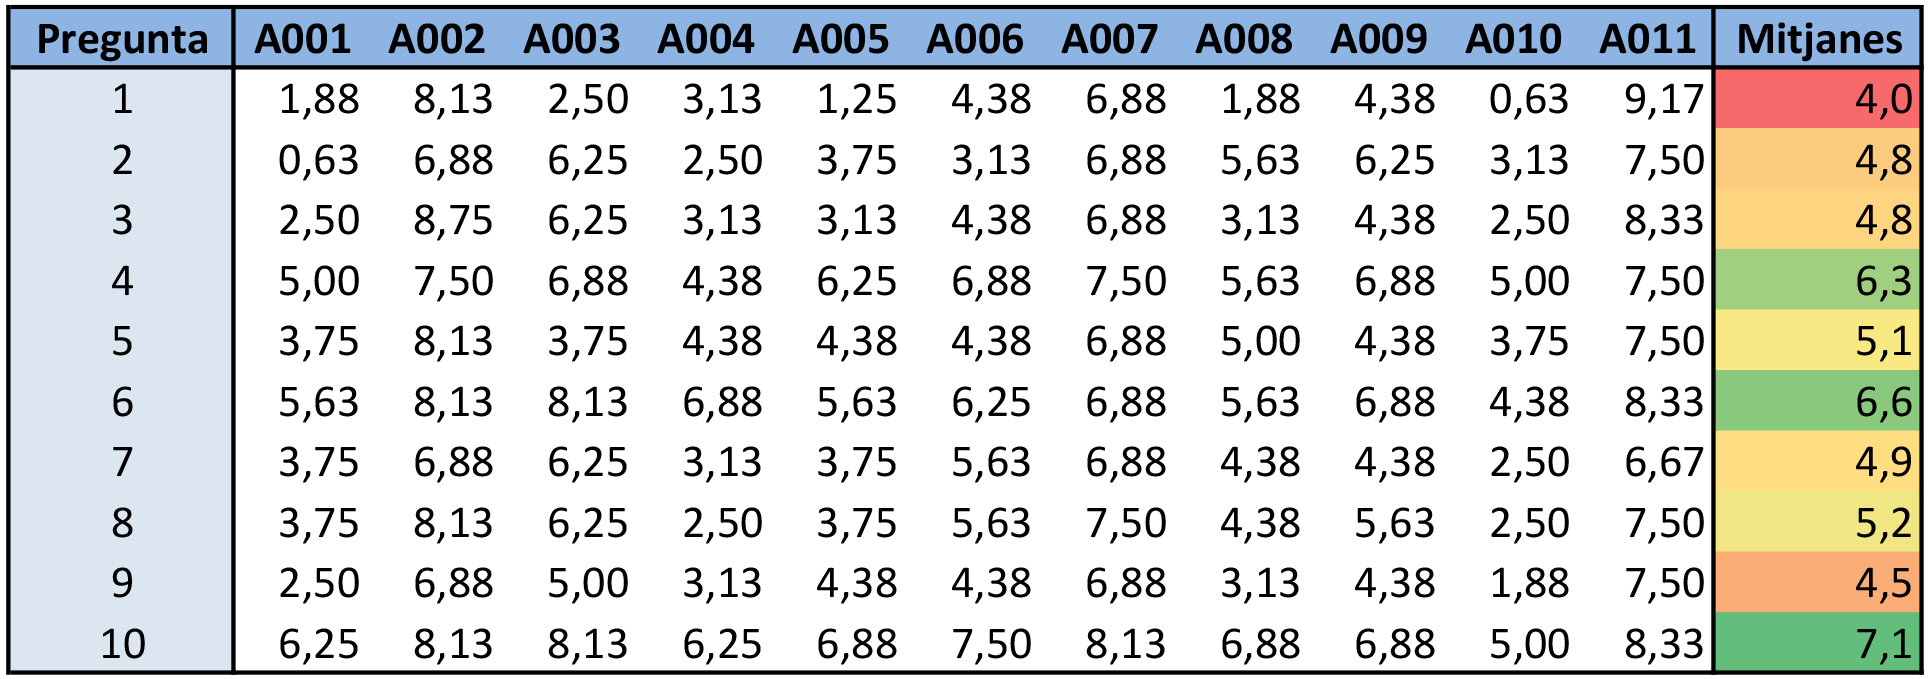
\includegraphics[scale=0.9]{SUS_table_2.png}
\caption{Resultats del questionari SUS per cada aplicació i cada pregunta}\label{fig:SUS_table}
\end{figure}

Com es pot comprovar les aplicacions que garanteixen una millor \ac{UX} són Expense Manager (A002), Money Lover (A007) i el Expensor beta (A011). És per això que s'han fet servir les 3 per fer un anàlisi amb més profunditat i amb més usuaris.

\subsubsection{Avaluació sumarial 2}
Partint de les 3 millor aplicacions de la primera part de l'avaluació sumarial (una d'elles és el prototip creat) s'ha deixat provar les aplicacions a X usuaris. %TODO change X
Després aquests usuaris han respost el qüestionari USE el qual és bastant més complet que el SUS. De cada aplicació s'ha fet la mitjana de tots els usuaris donant lloc a la puntuació de cada aplicació la qual, com al qüestionari SUS, està entre 0 i 100. Les puntuacions de les 3 aplicacions es poden veure a la figura \ref{fig:USE_1} i a la figura \ref{fig:USE_2} s'ha modificat l'eix vertical per a que es vegin millor les diferencies.

\begin{figure}
	\centering
	
	\begin{subfigure}[b]{0.45\textwidth}
		\centering
		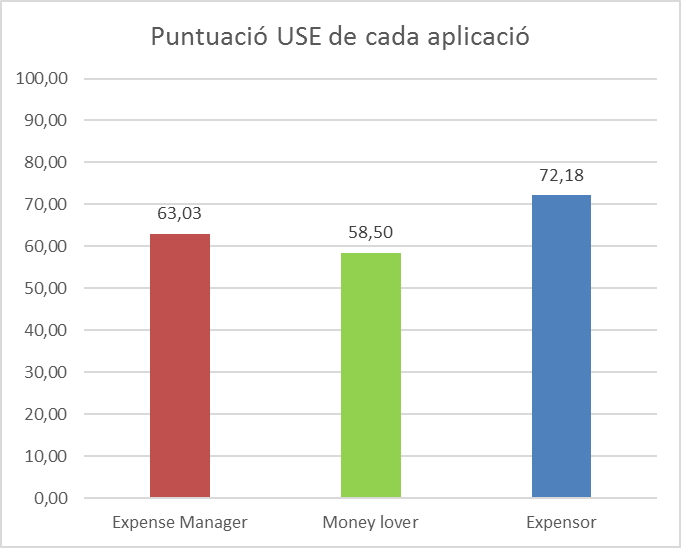
\includegraphics[scale=0.6]{USE_1.png}
		\caption{Resultats USE}
		\label{fig:USE_1}
	\end{subfigure}
	\quad
	\begin{subfigure}[b]{0.45\textwidth}
		\centering
		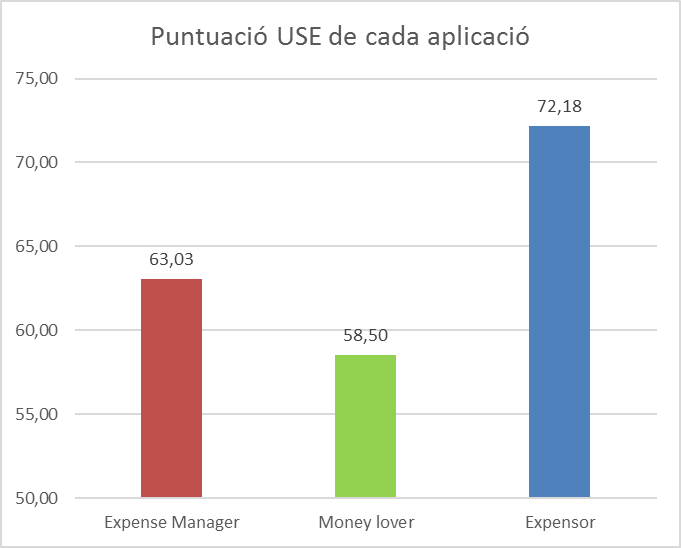
\includegraphics[scale=0.6]{USE_2.png}
		\caption{Resultats USE ampliat}
		\label{fig:USE_2}
	\end{subfigure}

\caption{Resultats del questionari USE per cada aplicació}\label{fig:USE_result}
\end{figure}

Com que el questionari USE està dividit en 4 seccions, s'ha calculat la nota de cada aplicació per cada secció (entre 0 i 10), veient així els punts forts i febles de cada aplicació. Es poden veure aquestes puntuacions a la figura \ref{fig:USE_2}

\begin{figure}[htp]
\centering
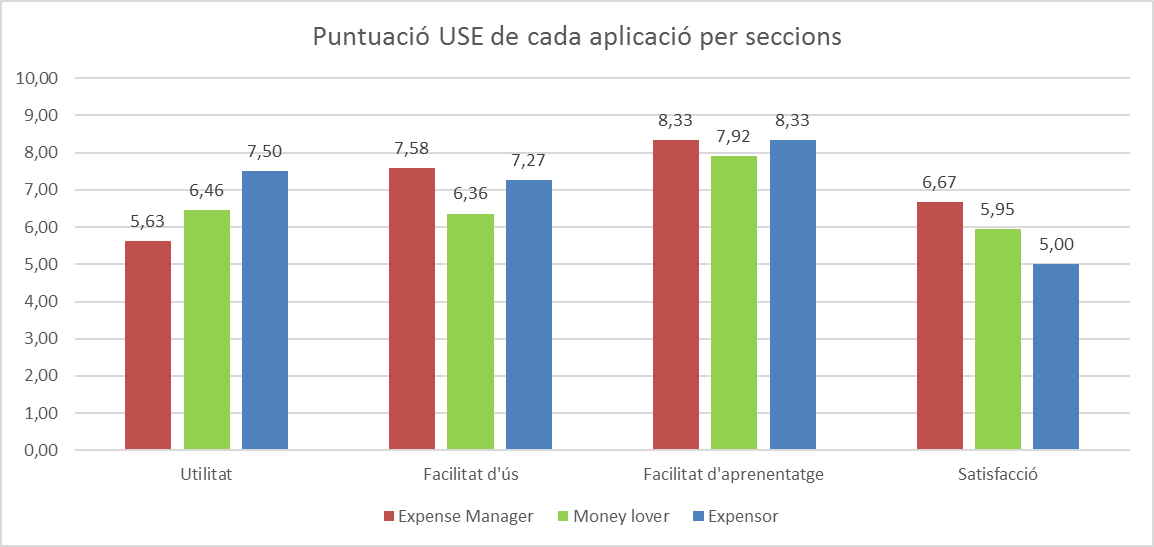
\includegraphics[scale=0.7]{USE_3.png}
\caption{Resultats del questionari USE de cada secció per cada aplicació}\label{fig:USE_2}
\end{figure}

\section{El procés iteratiu}
Les 4 etapes abans descrites no s'han dut a terme de forma lineal, sinó que s'ha seguit un procés iteratiu. Cronològicament l'estudi s'ha fet de la següent forma:

\begin{enumerate}
\item Anàlisi inicial amb les aplicacions ja existents
\item Disseny i anàlisi amb prototips de baixa fidelitat
\item Comprovar la validesa de l'anàlisi inicial
\item Disseny i anàlisi amb prototips de mitja fidelitat
\item Comprovar la validesa de l'anàlisi inicial
\item Disseny i anàlisi del prototip d'alta fidelitat, comparant-lo amb la resta d'aplicacions existents.
\end{enumerate}

\subsubsection{Disseny i anàlisi amb prototips de baixa fidelitat}
Aquesta iteració inclou els esbossos inicials i el prototip PH1. Al ser de baixa fidelitat només s'ha avaluat amb un grup reduït d'usuaris de confiança.
\subsubsection{Disseny i anàlisi amb prototips de mitja fidelitat}
En aquesta iteració s'han dissenyat els tres prototips de mitja fidelitat PH2, PV1 i PL1 mitjançant el programa \gls{Balsamiq_Mockups}. Per avaluar-los s'han fet 22 entrevistes als usuaris conduïdes amb una enquesta per a l'avaluació formativa.
\subsubsection{Disseny i anàlisi del prototip d'alta fidelitat}
En aquesta iteració s'ha creat un prototip completament programat. S'ha fet una primera avaluació sumarial amb un qüestionari curt (SUS), comparant-lo amb les altres aplicacions ja existents. Després s'ha fet una segona avaluació sumarial amb més profunditat del prototip final juntament amb les 2 millors aplicacions de l'avaluació sumarial anterior. 